%*****************************************
\chapter{Fundamental Skills}\label{ch01:fundamentals}
%*****************************************

Microsoft\textsuperscript{\textregistered} Excel\textsuperscript{\textregistered} is a tool that can be used in virtually all careers and is valuable in both professional and personal settings. Applications as diverse as keeping track of medications in inventory for a hospital or creating a financial plan for retirement can be done efficiently and accurately with Excel. This chapter introduces the fundamental skills necessary start with Excel. Most people find that learning only a few skills makes them very productive in a short period of time. 

\section{Overview of Microsoft Excel}

\begin{center}
	\begin{objbox}{Learning Objectives}
		\begin{itemize}
			\setlength{\itemsep}{0pt}
			\setlength{\parskip}{0pt}
			\setlength{\parsep}{0pt}
			
			\item Examine the value of using Excel to make decisions.
			\item Learn how to start Excel.
			\item Become familiar with the Excel workbook.
			\item Understand how to navigate worksheets.
			\item Examine the Excel Ribbon.
			\item Examine the right-click menu options.
			\item Learn how to save workbooks.
			\item Examine the Status Bar.
			\item Become familiar with the features in the Excel Help window.
			
		\end{itemize}
	\end{objbox}
\end{center}

Microsoft\textsuperscript{\textregistered} Office\textsuperscript{\textregistered} contains a variety of tools that help people accomplish many personal and professional objectives, but Excel is perhaps the most versatile and widely used of all the Office applications. Most career paths need to use Excel from time-to-time to accomplish professional objectives, often daily. This chapter provides an overview of the Excel application along with an orientation for accessing the commands and features of an Excel workbook.

\subsection{Making Decisions With Excel}

Taking a very simple view, Excel is a tool for entering quantitative data into an electronic spreadsheet to apply one or several mathematical computations. These computations ultimately convert that quantitative data into information. The information produced in Excel can be used to make decisions in both professional and personal contexts. For example, employees can use Excel to determine how much inventory to buy for a clothing retailer, how much medication to administer to a patient, or how to balance income with outgo. With respect to personal decisions, Excel can help determine how much money is available to spend on a house, car payment, or savings for retirement. This text demonstrates using Excel to make these decisions, and many more.

Figure \ref{01:fig01} shows a completed Excel worksheet that will be constructed in this chapter. The information shown in this worksheet is the top-line sales data for a hypothetical merchandise retail company. The worksheet data can help this retailer determine how many salespeople are needed for each month, how much inventory is needed to satisfy sales, and what types of products should be purchased.

\begin{figure}[H]
	\centering
	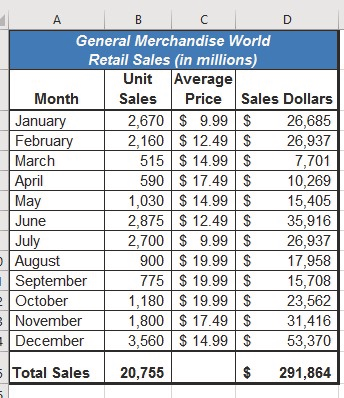
\includegraphics[width=\maxwidth{.95\linewidth}]{gfx/ch01_fig01}
	\caption{Example of an Excel Worksheet}
	\label{01:fig01}
\end{figure}

\subsection{Starting Excel}

\begin{enumerate}
	\item Locate Excel on the Windows menu.
	\item Click \fmtButton{Microsoft Excel} to launch the Excel application.
	\item Click the first option, \fmtButton{Blank Workbook}.
\end{enumerate}

\subsection{The Excel Workbook}

Once Excel is started, a blank workbook will open. A workbook is an Excel file that contains one or more worksheets (sometimes referred to as spreadsheets). Excel will assign a file name to the workbook, such as \textit{Book1}, \textit{Book2}, \textit{Book3}, and so on, depending on how many new workbooks are opened. Figure \ref{01:fig02} shows a blank workbook after starting Excel. Take some time to become familiar with this screen. (\textit{Note: the worksheet screen may be slightly different depending on the version of Excel being used.})

\begin{figure}[H]
	\centering
	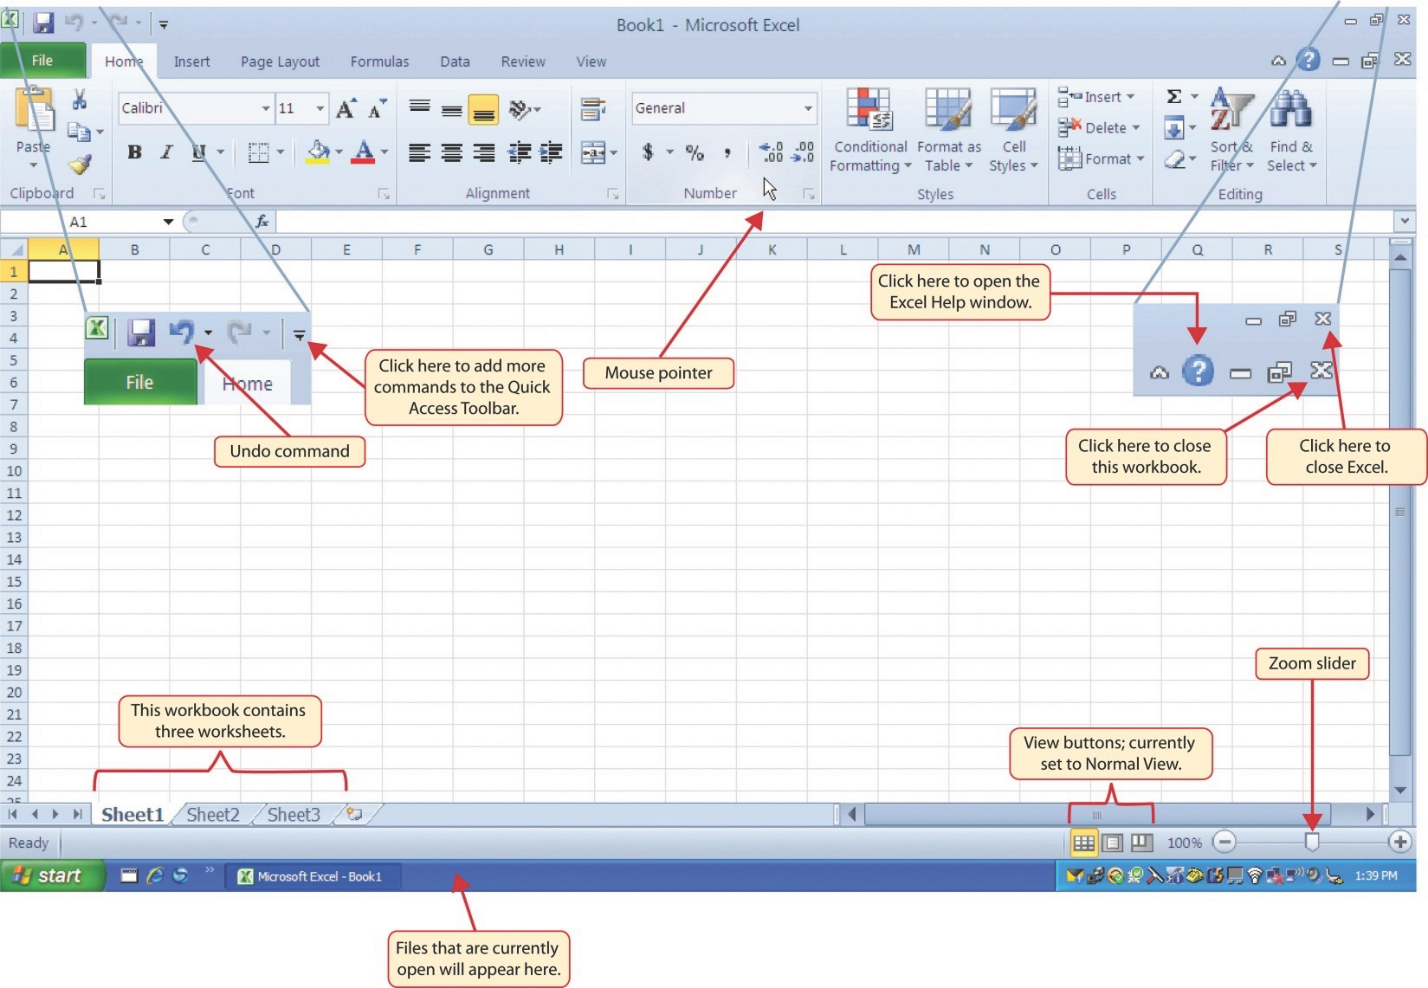
\includegraphics[width=\maxwidth{.95\linewidth}]{gfx/ch01_fig02}
	\caption{Blank Workbook}
	\label{01:fig02}
\end{figure}

The workbook should already be maximized (or shown at full size) once Excel is started, as shown in Figure \ref{01:fig02}. However, if the screen looks like Figure \ref{01:fig03} after starting Excel, click the \fmtButton{Maximize} button, as shown in the figure.

\begin{figure}[H]
	\centering
	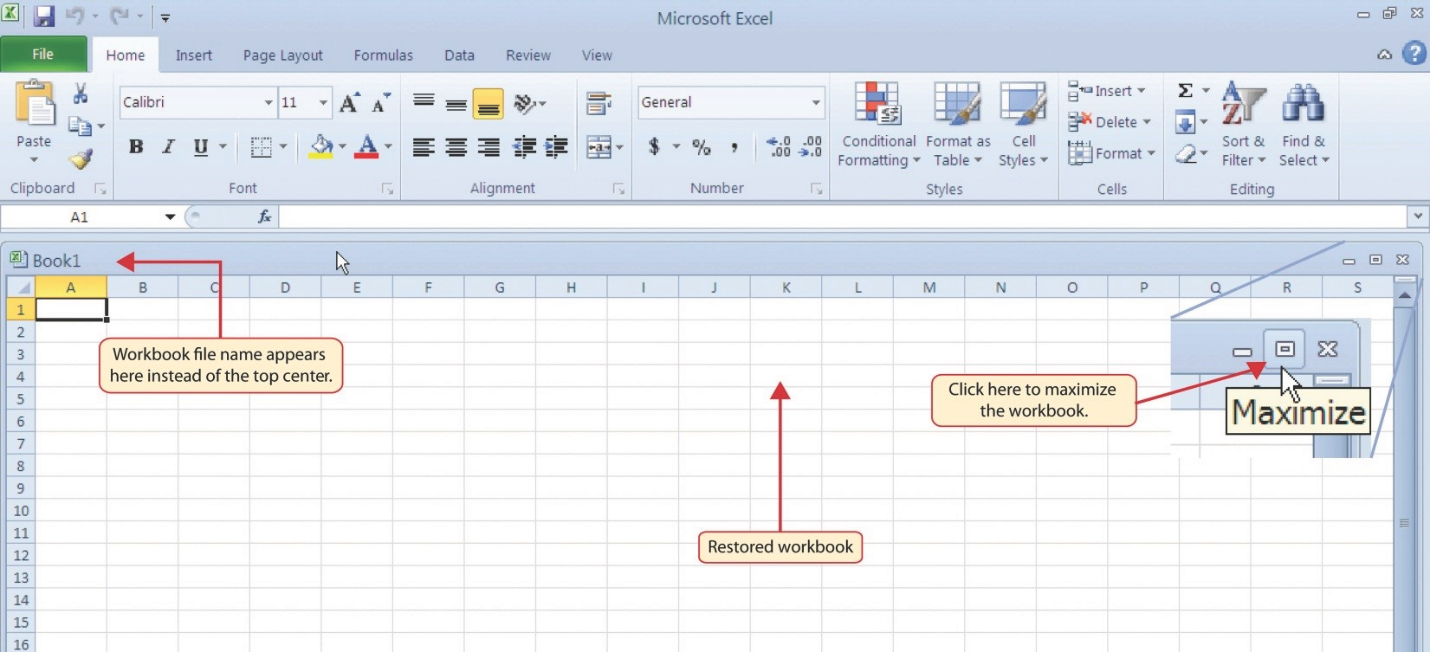
\includegraphics[width=\maxwidth{.95\linewidth}]{gfx/ch01_fig03}
	\caption{Restored Worksheet}
	\label{01:fig03}
\end{figure}

\subsection{Navigating Worksheets}

Data is entered and managed in an Excel worksheet. The worksheet contains several rectangles called cells for entering numeric and non-numeric data. Each cell in an Excel worksheet is located at an address, which is defined by a column letter followed by a row number. For example, the cell that is currently activated in Figure \ref{01:fig03} is $ A1 $. This would be referred to as cell location $ A1 $ or cell reference $ A1 $. The following steps explain how to navigate in an Excel worksheet.

\begin{itemize}
	\item Place the mouse pointer over cell \fmtLoc{D5} and left click.
	\item Check to make sure \fmtLoc{Column D} and \fmtLoc{Row 5} are highlighted, as shown in Figure \ref{01:fig04}.
\end{itemize}

\begin{figure}[H]
	\centering
	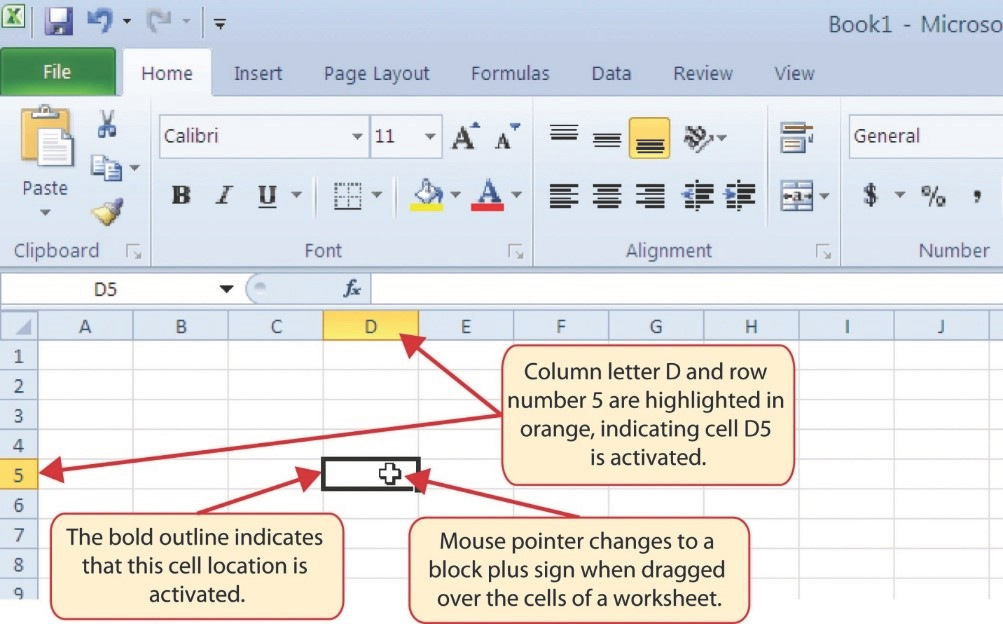
\includegraphics[width=\maxwidth{.95\linewidth}]{gfx/ch01_fig04}
	\caption{Activating a Cell Location}
	\label{01:fig04}
\end{figure}

\begin{enumerate}
	\item Click the mouse pointer in cell \fmtLoc{A1}.
	\item Click and hold the left mouse button and drag the mouse pointer back to cell \fmtLoc{D5}.
	\item Release the left mouse button. Several cells are now highlighted, as shown in Figure \ref{01:fig05}.
\end{enumerate}

\begin{figure}[H]
	\centering
	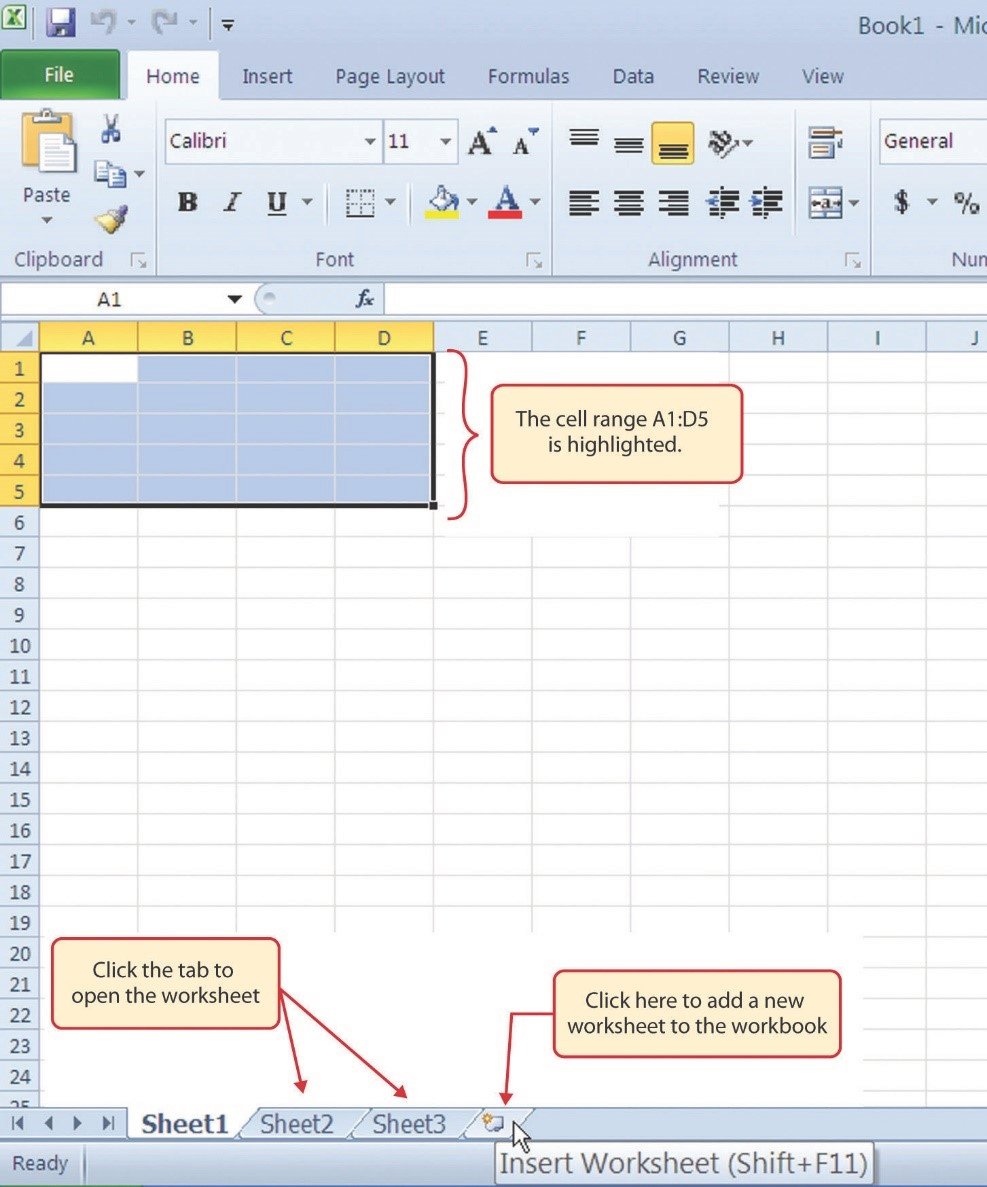
\includegraphics[width=\maxwidth{.95\linewidth}]{gfx/ch01_fig05}
	\caption{Highlighting a Range of Cells}
	\label{01:fig05}
\end{figure}

This is referred to as a cell range and is usually written as $ A1 $:$ D5 $. Any two cell locations separated by a colon are known as a cell range. The first cell in the range is the top left corner and the second cell is the lower right corner.

\begin{enumerate}
	\item At the bottom of the screen are tabs that identify different worksheets. Depending on the version of Excel being used there may be three as displayed in Figure \ref{01:fig05} or just one. If there is only one sheet, clicking \fmtButton{Insert Worksheet} adds a new worksheet. Different versions of Excel use \fmtButton{$ + $} or \fmtButton{Insert Worksheet} buttons. For this exercise, add worksheets as necessary so three are available.
	\item Click the \fmtWorksheet{Sheet1} tab at the bottom of the screen to activate it, as shown in Figure \ref{01:fig05}.
\end{enumerate}

\begin{center}
	\begin{shtcutbox}{Keyboard Shortcuts}
		\textbf{Basic Worksheet Navigation}
		\\
		\begin{itemize}
			\setlength{\itemsep}{0pt}
			\setlength{\parskip}{0pt}
			\setlength{\parsep}{0pt}

			\item Use the arrow keys on the keyboard to move the cell pointer to different cells on the worksheet.
			\item Hold the \fmtKeystroke{Shift} key and press the arrow keys on the keyboard to highlight a range of cells in a worksheet.
			\item Hold the \fmtKeystroke{Ctrl} key while pressing the \fmtKeystroke{Page Down} or \fmtKeystroke{Page Up} keys to open other worksheets in a workbook.

		\end{itemize}
	\end{shtcutbox}
\end{center}

\subsection{The Excel Ribbon}

Excel's features and commands are found in the \textit{Ribbon}, which is the upper area of the Excel screen that contains several tabs running across the top. Each tab provides access to a different set of Excel commands. Figure \ref{01:fig06} shows the commands available in the \textit{Home} tab of the Ribbon. Table \ref{01:tab01}, \textit{Command Overview for Each Tab of the Ribbon}, provides an overview of the commands that are found in each tab of the Ribbon.

\begin{figure}[H]
	\centering
	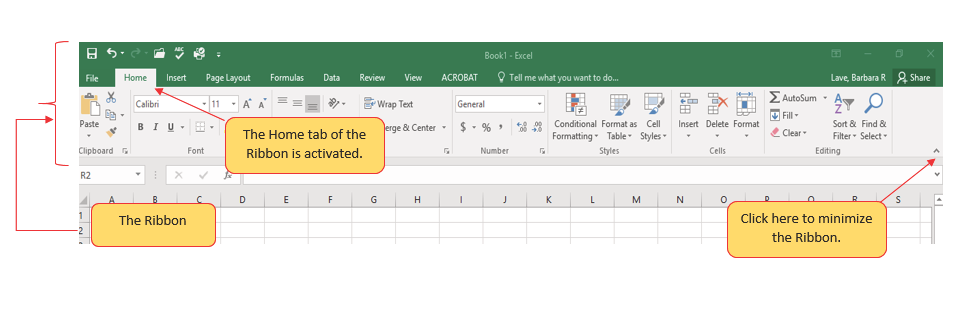
\includegraphics[width=\maxwidth{.95\linewidth}]{gfx/ch01_fig06}
	\caption{Home Tab of the Ribbon}
	\label{01:fig06}
\end{figure}

\begin{table}[H]
	\rowcolors{1}{}{tablerow} % zebra striping background
	{\small
		%\fontsize{8}{10} \selectfont %Replace small for special font size
		\begin{longtable}{L{0.75in}L{3.50in}} %Left-aligned, Max width: 4.25in
			\textbf{Tab} & \textbf{Description} \endhead
			\hline

			File & Also known as the \textit{Backstage View} of the Excel workbook. Contains all commands for opening, closing, saving, and creating new Excel workbooks. Includes print commands, document properties, e-mailing options, and help features. Excel's user options are also found in this tab.\\

			Home & Contains the most frequently used Excel commands. Formatting commands are found in this tab along with commands for cutting, copying, pasting, and for inserting and deleting rows and columns.\\
			
			Insert & Used to insert objects such as charts, pictures, shapes, PivotTables, Internet links, symbols, or text boxes.\\
			
			Page Layout & Contains commands used to prepare a worksheet for printing. Also includes commands used to show and print the grid lines on a worksheet.\\
			
			Formulas & Includes commands for adding mathematical functions to a worksheet. Also contains tools for auditing mathematical formulas.\\
			
			Data & Used when working with external data sources such as Microsoft® Access®, text files, or the Internet. Also contains sorting commands and access to scenario tools.\\
			
			Review & Includes Spelling and Track Changes features. Also contains protection features to password protect worksheets or workbooks.\\
			
			View & Used to adjust the visual appearance of a workbook. Common commands include the Zoom and Page Layout view.\\

			\rowcolor{captionwhite}
			\caption{Command Overview for Ribbon Tabs}
			\label{01:tab01}
		\end{longtable}
	} % End small
\end{table}

The Ribbon shown in Figure \ref{01:fig06} is full, or maximized. The benefit of having a full Ribbon is that the commands are always visible while developing a worksheet. However, depending on the screen dimensions of the computer, the Ribbon may take up too much vertical space on the worksheet. If this is the case, it can be minimized by clicking the button shown in Figure \ref{01:fig06}. When minimized, the Ribbon will show only the tabs and not the command buttons. Clicking a tab makes the command buttons appear until a command is selected or the mouse is clicked anywhere on the worksheet. Once the ribbon is expanded it can be pinned open by clicking the \fmtButton{pin} button at the lower left corner of the ribbon.

\begin{center}
	\begin{shtcutbox}{Keyboard Shortcuts}
		\textbf{Minimizing or Maximizing the Ribbon}
		\\
		\begin{itemize}
			\setlength{\itemsep}{0pt}
			\setlength{\parskip}{0pt}
			\setlength{\parsep}{0pt}
			
			\item Hold down the \fmtKeystroke{Ctrl} key and press the \fmtKeystroke{F1} key to toggle between the maximized and minimized view of the ribbon.
			
		\end{itemize}
	\end{shtcutbox}
\end{center}

\subsection{Quick Access Toolbar and Right-Click Menu}

The \textit{Quick Access Toolbar} is found at the upper left side of the Excel screen above the Ribbon, as shown in Figure \ref{01:fig07}. This area provides access to the most frequently used commands, such as Save and Undo. The \textit{Quick Access Toolbar} can be customized by adding commands that are regularly used. By placing these commands in the \textit{Quick Access Toolbar}, it is not necessary to navigate through the Ribbon to find them. To customize the \textit{Quick Access Toolbar}, click the down arrow as shown in Figure \ref{01:fig07}. This will open a menu of commonly-used commands that can be added to the \textit{Quick Access Toolbar}. If the desired command is not on the list, select the \textit{More Commands} option, which opens a screen containing every command on the ribbon.

\begin{figure}[H]
	\centering
	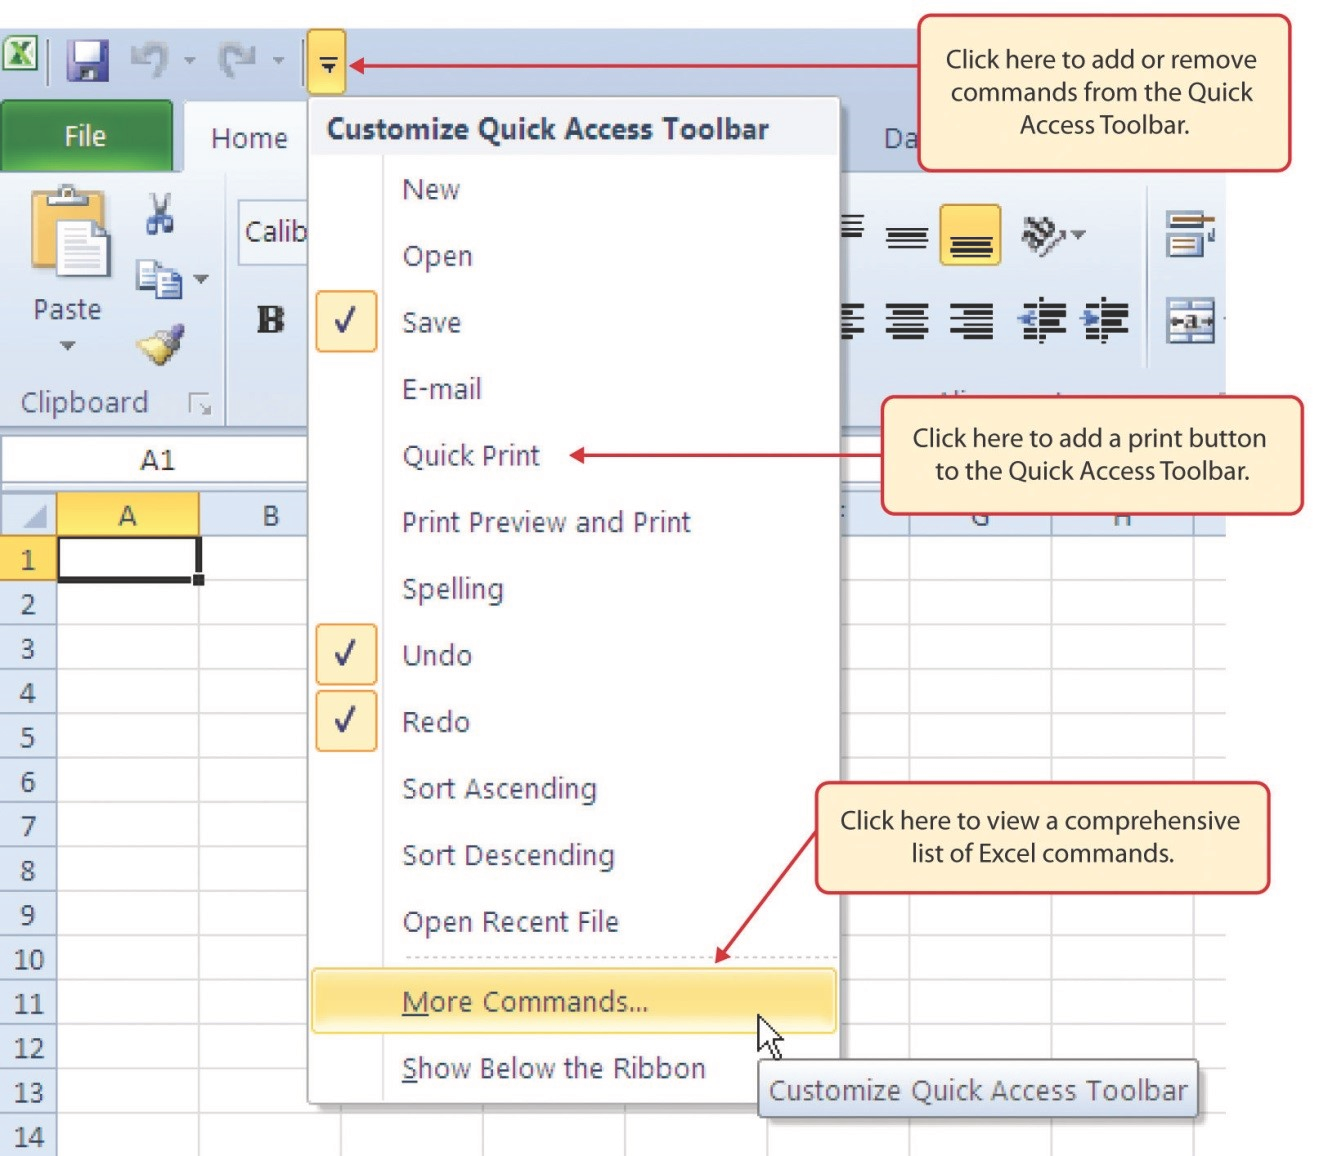
\includegraphics[width=\maxwidth{.95\linewidth}]{gfx/ch01_fig07}
	\caption{Customizing the Quick Access Toolbar}
	\label{01:fig07}
\end{figure}

In addition to the Ribbon and Quick Access Toolbar, commands can also be accessed by right-clicking anywhere on the worksheet and opening a context menu. \ref{01:fig08} shows an example of the commands available in the context menu.

\begin{figure}[H]
	\centering
	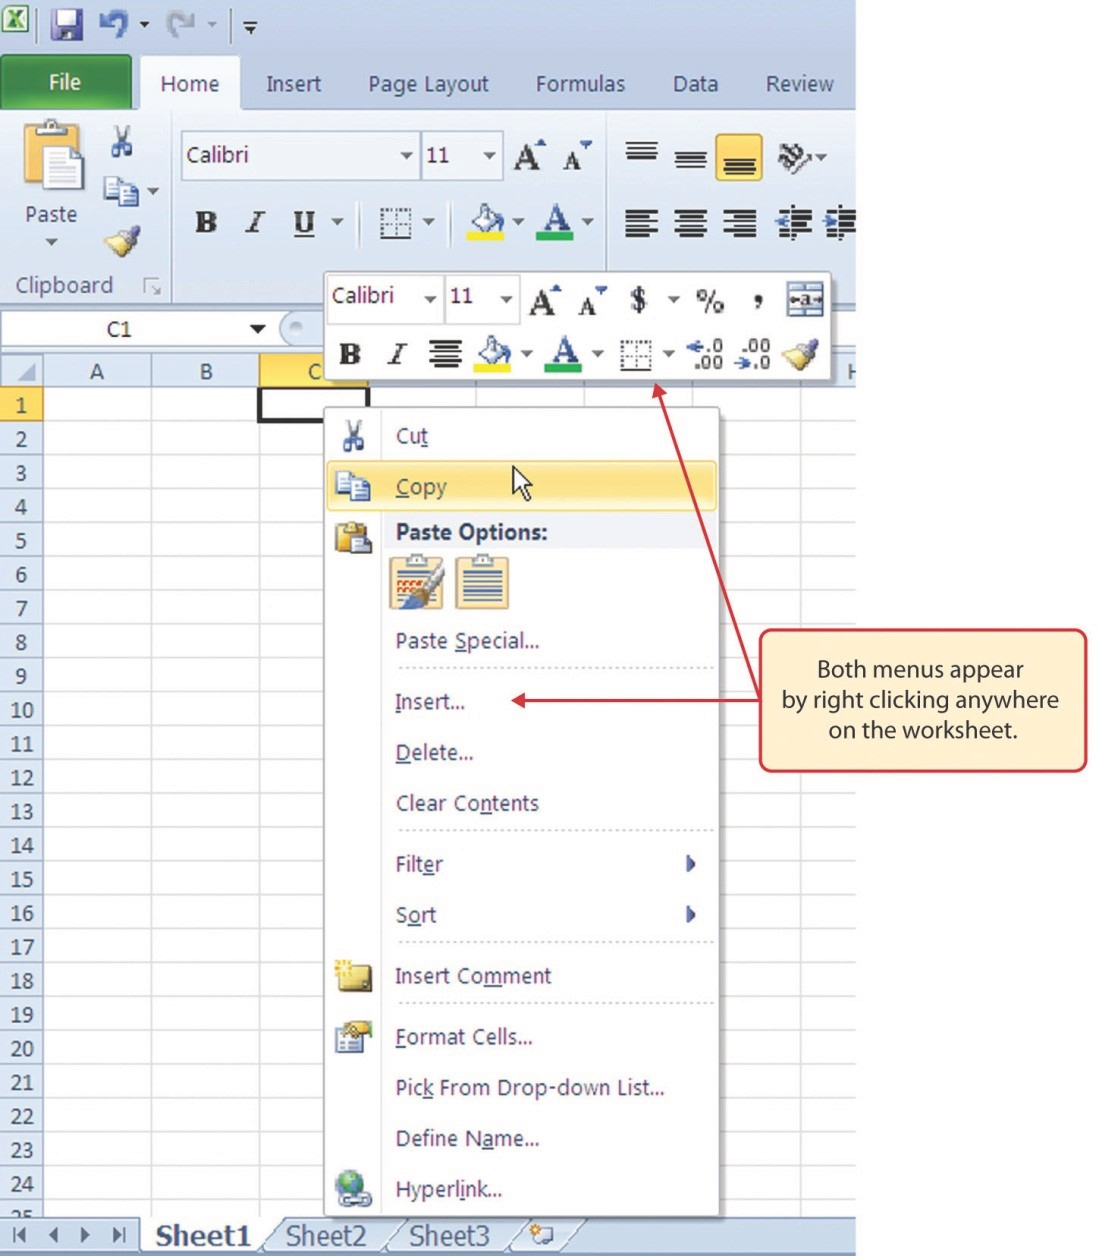
\includegraphics[width=\maxwidth{.95\linewidth}]{gfx/ch01_fig08}
	\caption{Right-Click Menu}
	\label{01:fig08}
\end{figure}

\subsection{The File Tab}

The \textit{File} tab is also known as the \textit{Backstage} view of the workbook. It contains a variety of features and commands related to the workbook that is currently open, new workbooks, or workbooks stored in other locations on the computer or network. Figure \ref{01:fig09} shows the options available in the \textit{File} tab or \textit{Backstage} view. To leave the \textit{Backstage} view and return to the worksheet, click the arrow in the upper left-hand corner as shown in Figure \ref{01:fig09}.

\begin{figure}[H]
	\centering
	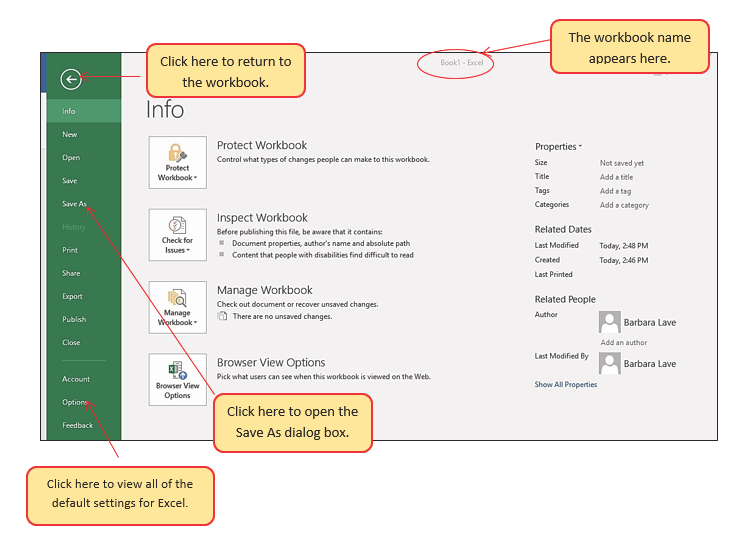
\includegraphics[width=\maxwidth{.95\linewidth}]{gfx/ch01_fig09}
	\caption{File Tab or Backstage View of a Workbook}
	\label{01:fig09}
\end{figure}

Included in the \textit{File} tab are the numerous Excel settings that can be accessed and modified by clicking the \textit{Options} button. Figure \ref{01:fig10} shows the Excel \textit{Options} window, which opens access to settings such as the default font style, font size, and the number of worksheets that appear in new workbooks. Chapter \ref{ch09:topics}, \nameref{ch09:topics}, page \pageref{ch09:topics}, has more information about setting common options.

\begin{figure}[H]
	\centering
	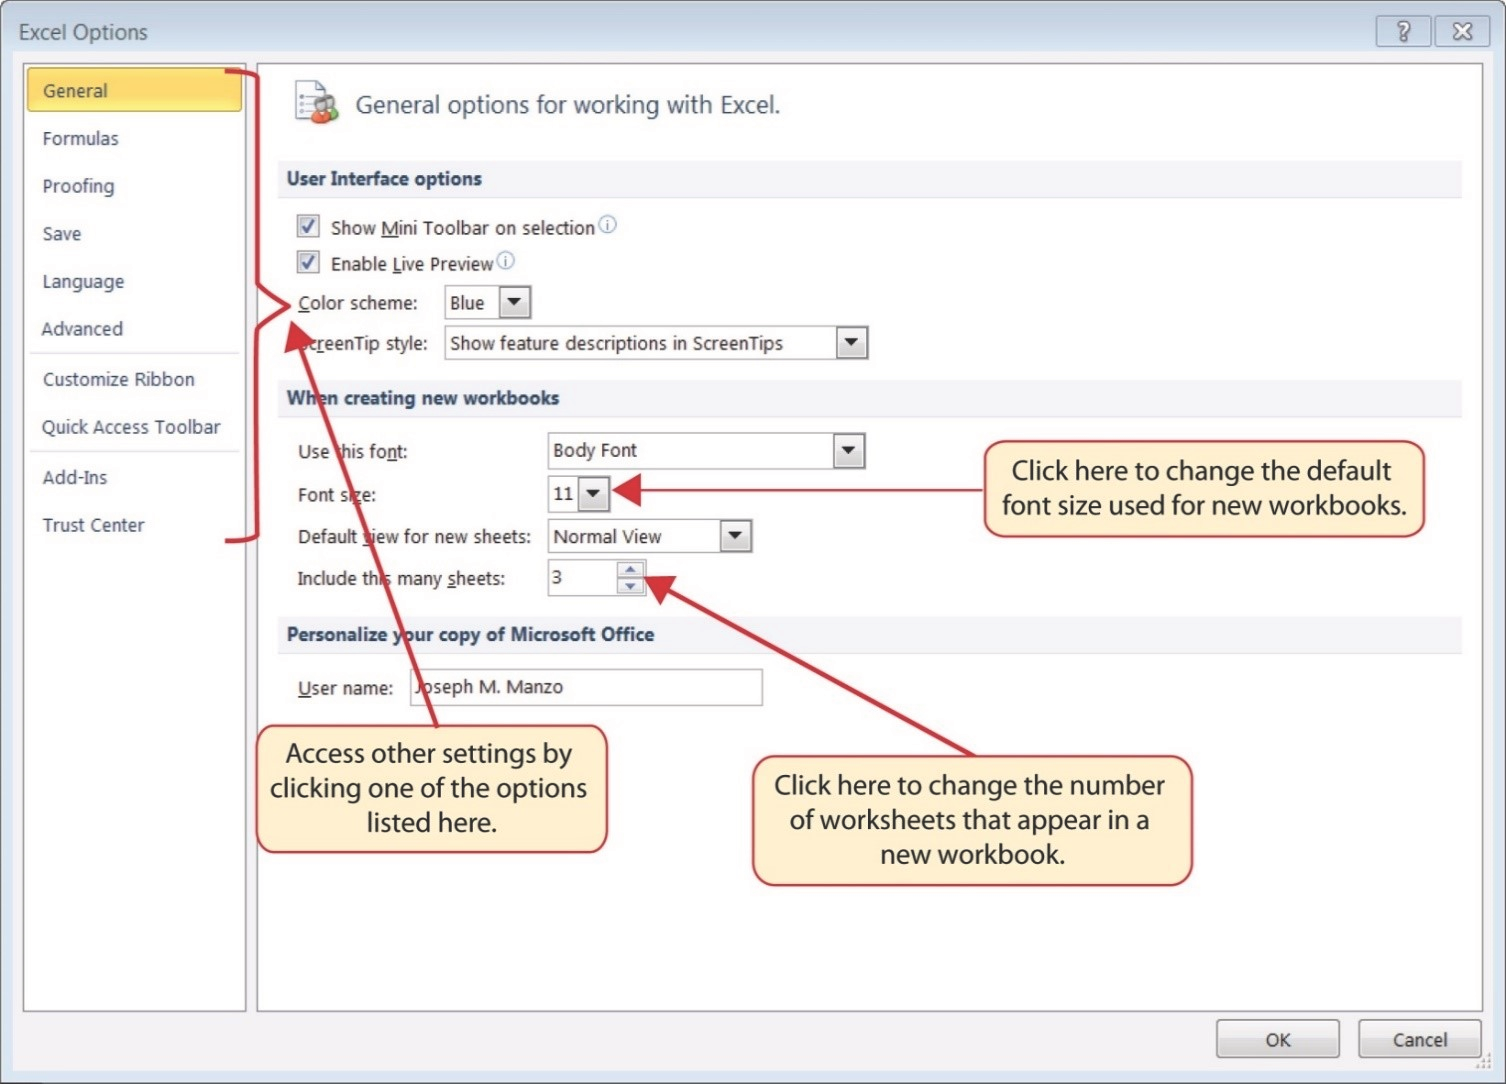
\includegraphics[width=\maxwidth{.95\linewidth}]{gfx/ch01_fig10}
	\caption{Excel Options Window}
	\label{01:fig10}
\end{figure}

\subsection{Saving Workbooks (Save As)}

Once a new workbook is created, the file name needs to be specified and a location chosen on the computer or network to save that file. A blank workbook was opened earlier in this lesson and it should now be saved. It is important to remember where the workbook is saved since it will be used later in this chapter to construct the workbook shown in Figure \ref{01:fig01}. As a tip, it is probably easiest to store all workbooks used in this course in the same folder.

\begin{enumerate}[resume]
	\item Click \fmtButton{File $ \Rightarrow $ Save As}. This will open the \textit{Save As} dialog.
	\item Determine a location for saving on the computer by clicking \fmtButton{Browse} on the left side to open the \textit{Save As} dialog box as illustrated in Figure \ref{01:fig12}.
	\item Click in the \textit{File Name} box near the bottom of the \textit{Save As} dialog box. Type the new file name: \fmtTyping{CH1-GMW Sales Data}
	\item Review the settings in the screen for correctness and click the \fmtButton{Save} button.
\end{enumerate}

\begin{figure}[H]
	\centering
	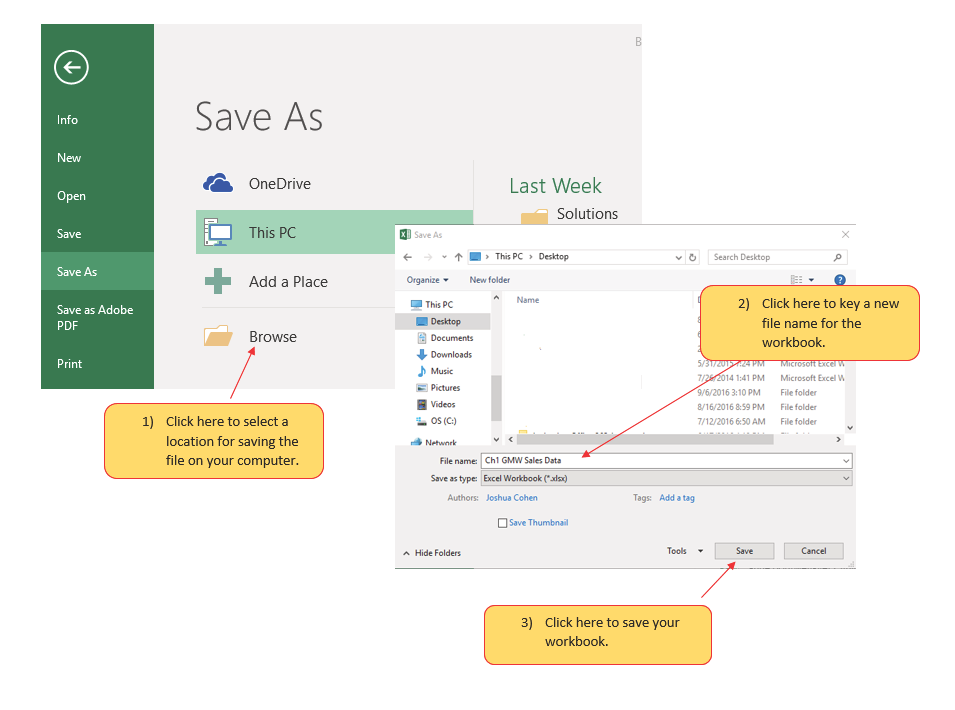
\includegraphics[width=\maxwidth{.95\linewidth}]{gfx/ch01_fig12}
	\caption{Save As Dialog in Excel}
	\label{01:fig12}
\end{figure}

\begin{center}
	\begin{shtcutbox}{Keyboard Shortcuts}
		\textbf{Save As}
		\\
		\begin{itemize}
			\setlength{\itemsep}{0pt}
			\setlength{\parskip}{0pt}
			\setlength{\parsep}{0pt}
			
			\item Press the \fmtKeystroke{F12} key and use the tab and arrow keys to navigate around the \textit{Save As} dialog box. Use the \fmtKeystroke{Enter} key to make a selection.
			\item Or press the \fmtKeystroke{Alt} key on the keyboard and Key Tips, small letters and numbers, appear on the Ribbon. Press the \fmtKeystroke{F} key on the keyboard for the \fmtButton{File} tab and then the \fmtKeystroke{A} key. This will open the \textit{Save As} dialog box.
			
		\end{itemize}
	\end{shtcutbox}
\end{center}

\begin{center}
	\begin{sklbox}{Skill Refresher}
		\textbf{Saving Workbooks (Save As)}
		\\
		\begin{itemize}
			\setlength{\itemsep}{0pt}
			\setlength{\parskip}{0pt}
			\setlength{\parsep}{0pt}
			
			\item Click the \fmtButton{File} tab on the Ribbon.
			\item Click the \fmtButton{Save As} option.
			\item Select a location on the computer.
			\item Click in the \textit{File} name box and type a new file name if needed.
			\item Click \fmtButton{Save as type $ \Rightarrow $ Down Arrow} and select the appropriate file type if needed.
			\item Click the \fmtButton{Save} button.
		
		\end{itemize}
	\end{sklbox}
\end{center}

\subsection{The Status Bar}

The Status Bar is located below the worksheet tabs on the Excel screen (see Figure \ref{01:fig13}). It displays a variety of information, such as the status of certain keys on the keyboard (\eg, CAPS LOCK), the available views for a workbook, the magnification of the screen, and mathematical functions that can be performed when data are highlighted on a worksheet. The Status Bar can be customized as follows.

\begin{enumerate}
	\item Place the mouse pointer over any area of the Status Bar and right-click to display the \textit{Customize Status Bar} list of options (see Figure \ref{01:fig13}).
	\item Select the \fmtButton{Caps Lock} option from the menu (see Figure \ref{01:fig13}).
	\item Press the \fmtKeystroke{Caps Lock} key on the keyboard and notice the Caps Lock indicator on the lower left side of the Status Bar.
	\item Press the \fmtKeystroke{Caps Lock} on the keyboard again. The indicator on the Status Bar goes away.
\end{enumerate}

\begin{figure}[H]
	\centering
	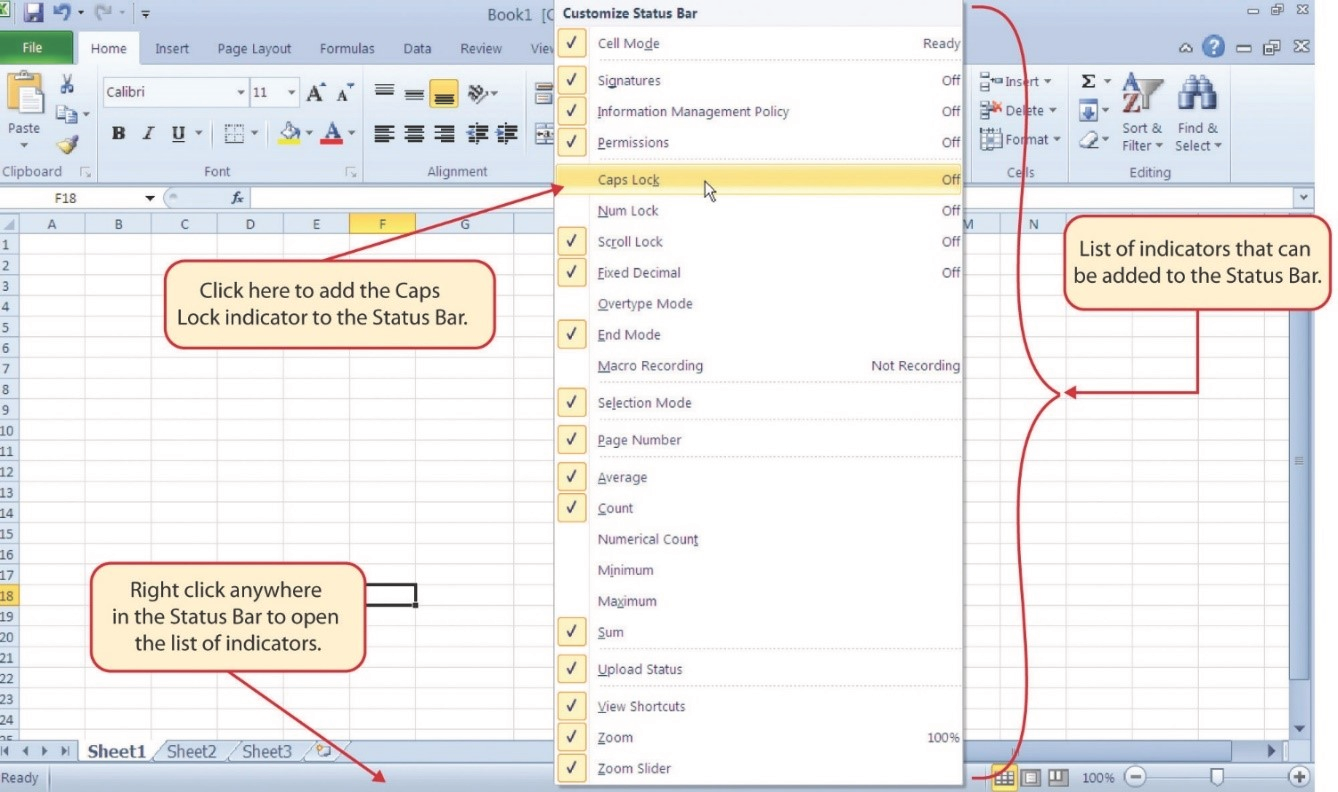
\includegraphics[width=\maxwidth{.95\linewidth}]{gfx/ch01_fig13}
	\caption{Customizing the Status Bar}
	\label{01:fig13}
\end{figure}

\subsection{Excel Help}

The Help feature provides extensive information about the Excel application. Although some of this information may be stored on the local computer, the Help window will automatically connect to the Internet if there is a live connection to provide resources that can answer most questions. 

Excel \fmtOldExcel{2016}. To access help, enter a question in the \textit{Tell me what you want to do} text box above the ribbon. A drop-down list with links to several potential answers will appear. Select from the links or click the question mark to launch the Excel Help window.

Excel \fmtNewExcel{365}. The Excel Help window can be opened by clicking the \fmtButton{Help} tab. Alternatively, enter a question in the \textit{Search} text box above the ribbon. A drop-down list with links to several potential answers will appear. Select from the links or click the question mark to launch the Excel Help window.

\begin{figure}[H]
	\centering
	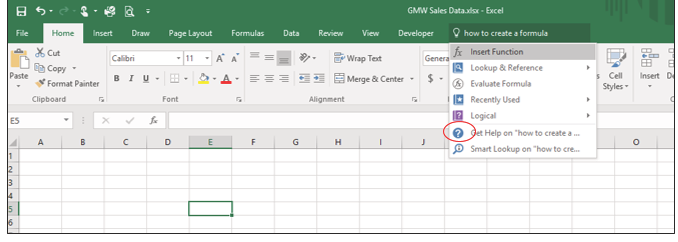
\includegraphics[width=\maxwidth{.95\linewidth}]{gfx/ch01_fig14}
	\caption{Excel Help Window}
	\label{01:fig14}
\end{figure}

\begin{center}
	\begin{shtcutbox}{Keyboard Shortcuts}
		\textbf{Excel Help}
		\\
		\begin{itemize}
			\setlength{\itemsep}{0pt}
			\setlength{\parskip}{0pt}
			\setlength{\parsep}{0pt}
			
			\item Press the \fmtKeystroke{F1} key on the keyboard.
			
		\end{itemize}
	\end{shtcutbox}
\end{center}


\begin{center}
	\begin{tkwbox}{Key Take-Aways}
		\textbf{Overview}
		\\
		\begin{itemize}
			\setlength{\itemsep}{0pt}
			\setlength{\parskip}{0pt}
			\setlength{\parsep}{0pt}
			
			\item Excel is a powerful tool for processing data for the purposes of making decisions.
			\item Excel commands are found throughout the tabs in the Ribbon.
			\item The \textit{Quick Access Toolbar} can be customized by adding frequently-used commands.
			\item Information displayed on the Status Bar can be customized.
			\item The Help window provides extensive information about Excel.
			
		\end{itemize}
	\end{tkwbox}
\end{center}

\section{Entering, Editing, and Managing Data}

\begin{center}
	\begin{objbox}{Learning Objectives}
		\begin{itemize}
			\setlength{\itemsep}{0pt}
			\setlength{\parskip}{0pt}
			\setlength{\parsep}{0pt}
			
			\item Understand how to enter data into a worksheet.
			\item Examine how to edit data in a worksheet.
			\item Examine how the Auto Fill Handle is used when entering data.
			\item Understand how to delete data from a worksheet and use the Undo command.
			\item Examine how to adjust column widths and row heights in a worksheet.
			\item Understand how to hide columns and rows in a worksheet.
			\item Examine how to insert columns and rows into a worksheet.
			\item Understand how to delete columns and rows from a worksheet.
			\item Learn how to move data to different locations in a worksheet.

		\end{itemize}
	\end{objbox}
\end{center}

This section begins the development of the workbook shown in Figure \ref{01:fig01}. The skills covered in this section are typically used in the early stages of developing one or more worksheets in a workbook.

\subsection{Entering Data}

Begin building the workbook shown in Figure \ref{01:fig01} by manually entering data into the worksheet. Begin by entering the column headings in \textit{Row 2}.

\begin{enumerate}
	\item Click cell location \fmtLoc{A2} on the worksheet.
	\item Type the word \fmtTyping{Month}.
	\item Press the \fmtKeystroke{Tab} key. This will enter the word into cell \fmtLoc{A2} and activate the next cell to the right.
	\item Type \fmtTyping{Unit Sales} and press the \fmtKeystroke{Tab} key.
	\item Repeat the above step for the words \fmtTyping{Average Price} and then again for \fmtTyping{Sales Dollars}.
\end{enumerate}

Figure \ref{01:fig15} shows how the worksheet should appear after the column headings have been entered into \textit{Row 2}. Notice that the word \textit{Price} in cell location $ C2 $ is not visible. This is because the column is too narrow to fit the entry. This will be corrected in the next section.

\begin{figure}[H]
	\centering
	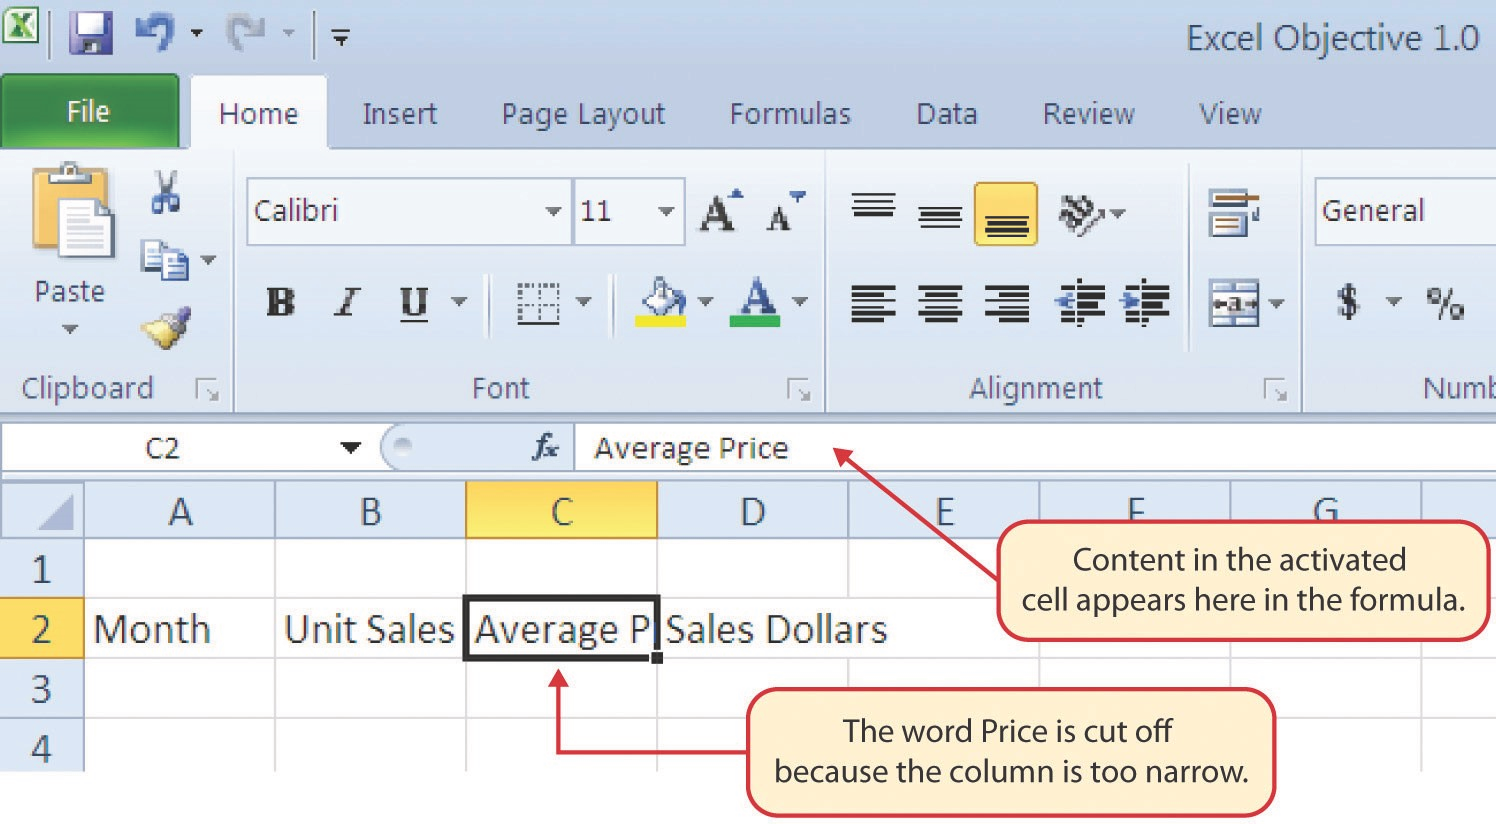
\includegraphics[width=\maxwidth{.95\linewidth}]{gfx/ch01_fig15}
	\caption{Entering Column Headings into a Worksheet}
	\label{01:fig15}
\end{figure}

\begin{center}
	\begin{infobox}{Integrity Check}
		\textbf{Column Headings}
		\\
		\\
		It is critical to include column headings that accurately describe the data in each column of a worksheet. In professional environments, Excel workbooks are commonly shared among coworkers. Good column headings reduce the chance of someone misinterpreting the data contained in a worksheet, which could lead to costly errors.
	\end{infobox}
\end{center}

\begin{enumerate}
	\item Click cell location \fmtLoc{B3}.
	\item Type the number \fmtTyping{$ 2670 $} and press the \fmtKeystroke{Enter} key. After pressing the \fmtKeystroke{Enter} key, cell \fmtLoc{B4} will be activated. Using the \fmtKeystroke{Enter} key is an efficient way to enter data vertically down a column.
	\item Enter the following numbers in cells \fmtLoc{B4} through \fmtLoc{B14}: \fmtTyping{$ 2160 $}, \fmtTyping{$ 515 $}, \fmtTyping{$ 590 $}, \fmtTyping{$ 1030 $}, \fmtTyping{$ $ 2875 $ $}, \fmtTyping{$ 2700 $}, \fmtTyping{$ 900 $}, \fmtTyping{$ 775 $}, \fmtTyping{$ 1180 $}, \fmtTyping{$ 1800 $}, and \fmtTyping{$ 3560 $}.
	\item Click cell location \fmtLoc{C3}.
	\item Type the number \fmtTyping{$ 9.99 $} and press the \fmtKeystroke{Enter} key.
	\item Enter the following numbers in cells \fmtLoc{C4} through \fmtLoc{C14}: \fmtTyping{$ 12.49 $}, \fmtTyping{$ 14.99 $}, \fmtTyping{$ 17.49 $}, \fmtTyping{$ 14.99 $}, \fmtTyping{$ 12.49 $}, \fmtTyping{$ 9.99 $}, \fmtTyping{$ 19.99 $}, \fmtTyping{$ 19.99 $}, \fmtTyping{$ 19.99 $}, \fmtTyping{$ 17.49 $}, and \fmtTyping{$ 14.99 $}.
	\item Click in cell \fmtLoc{D3}.
	\item Type the number \fmtTyping{$ 26685 $} and press the \fmtKeystroke{Enter} key.
	\item Enter the following numbers in cells \fmtLoc{D4} through \fmtLoc{D14}: \fmtTyping{$ 26937 $}, \fmtTyping{$ 7701 $}, \fmtTyping{$ 10269 $}, \fmtTyping{$ 15405 $}, \fmtTyping{$ 35916 $}, \fmtTyping{$ 26937 $}, \fmtTyping{$ 17958 $}, \fmtTyping{$ 15708 $}, \fmtTyping{$ 23562 $}, \fmtTyping{$ 31416 $}, and \fmtTyping{$ 53370 $}.
	\item When finished, check that the data entered matches Figure \ref{01:fig16}.
\end{enumerate}

\begin{figure}[H]
	\centering
	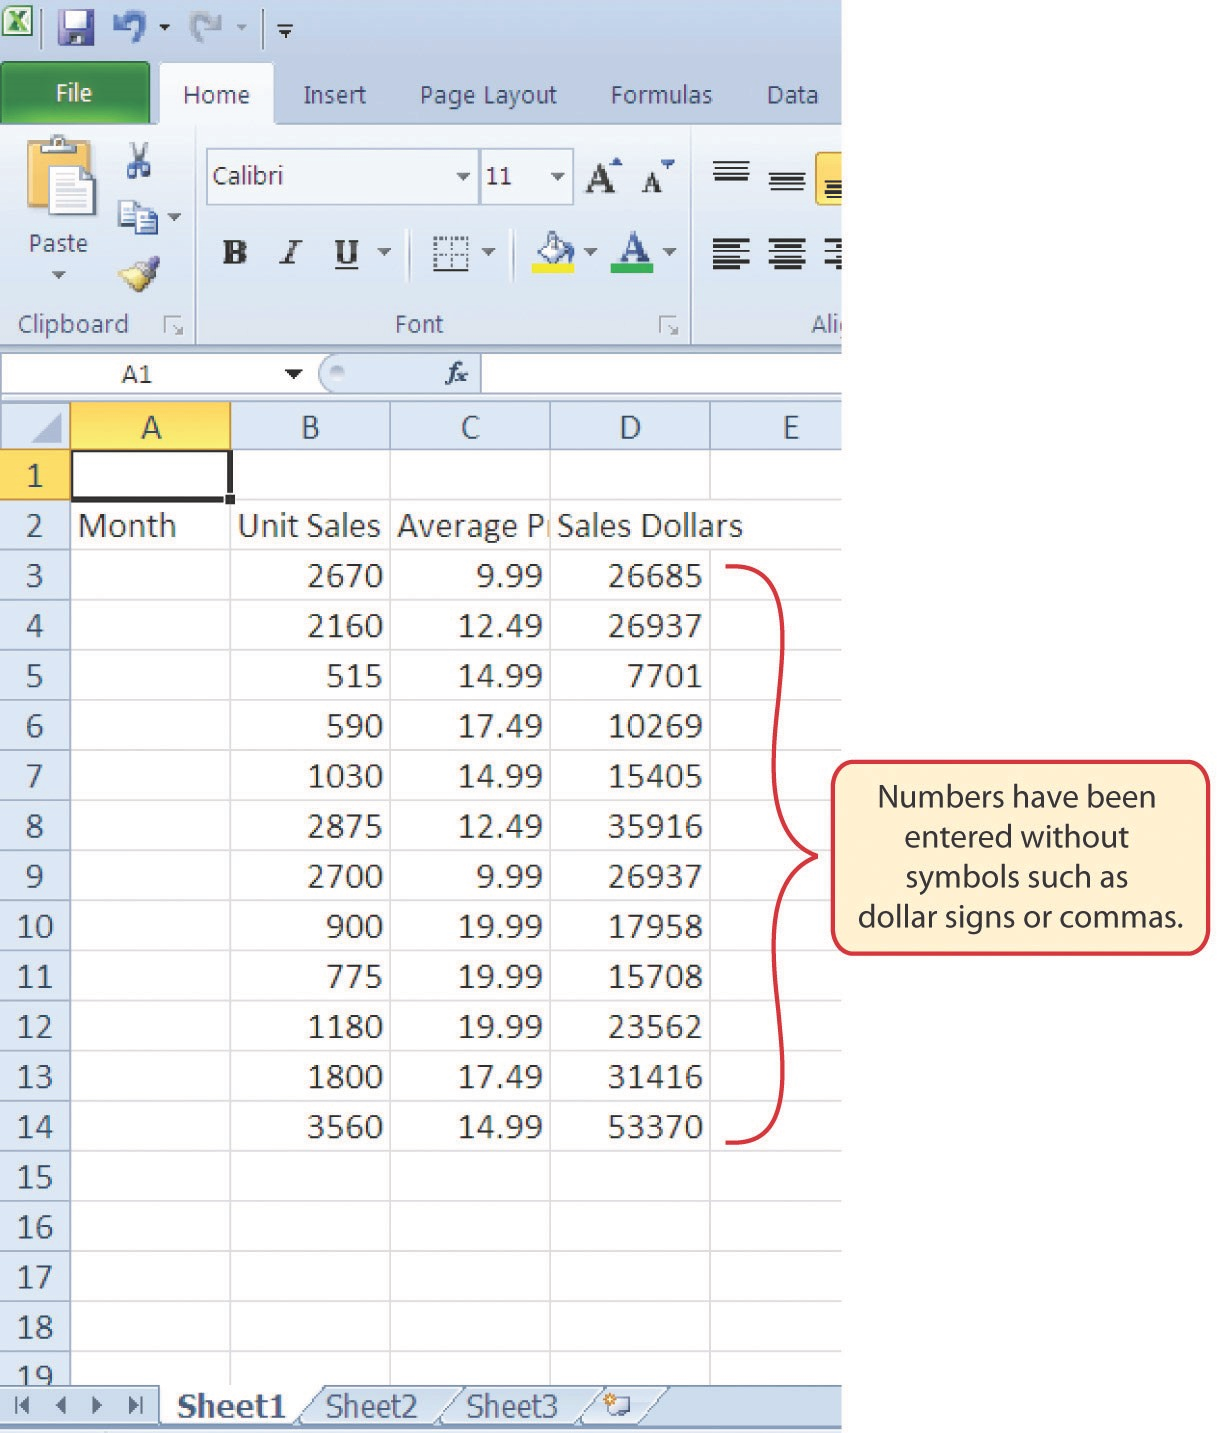
\includegraphics[width=\maxwidth{.95\linewidth}]{gfx/ch01_fig16}
	\caption{Completed Data Entry for Columns B, C, and D}
	\label{01:fig16}
\end{figure}

\begin{center}
	\begin{infobox}{Integrity Check}
		\textbf{Data Entry}
		\\
		\\
		One of the most likely points of error in any spreadsheet project is inaccurate data entry. When entering row and row of numbers it is easy to transpose or skip digits. Carefully checking data entry will reduce confusing results during the analysis phase of the project.
	\end{infobox}
\end{center}

\begin{center}
	\begin{infobox}{Why?}
		\textbf{Avoid Formatting Symbols When Entering Numbers}
		\\
		\\
		When typing numbers into an Excel worksheet, it is best to avoid adding any formatting symbols such as dollar signs and commas. Although Excel allows these symbols to be included while typing numbers, it slows down the process of entering data. It is more efficient to use Excel's formatting features to add these symbols to numbers after they are typed into a worksheet.
	\end{infobox}
\end{center}

\subsection{Editing Data}

Data that has been entered in a cell can be changed by double clicking the cell location or using the Formula Bar. The Formula Bar can be used for initial entery of data into cells as well as for editing data that already exists in a cell. The following steps provide an example of entering and then editing data that has been entered into a cell location.

\begin{enumerate}
	\item Click cell \fmtLoc{A15} in the \fmtWorksheet{Sheet1} worksheet.
	\item Type the abbreviation \fmtTyping{Tot} and press the \fmtKeystroke{Enter} key.
	\item Click cell \fmtLoc{A15}.
	\item Move the mouse pointer up to the Formula Bar. Notice that the pointer turns into a cursor. Move the cursor to the end of the abbreviation \textit{Tot} and left click.
	\item Type the letters \fmtTyping{al} to complete the word \textit{Total}.
	\item Click the checkmark to the left of the Formula Bar (see Figure \ref{01:fig17}) or press the \fmtKeystroke{Enter} key to enter the change into the cell.
\end{enumerate}

\begin{figure}[H]
	\centering
	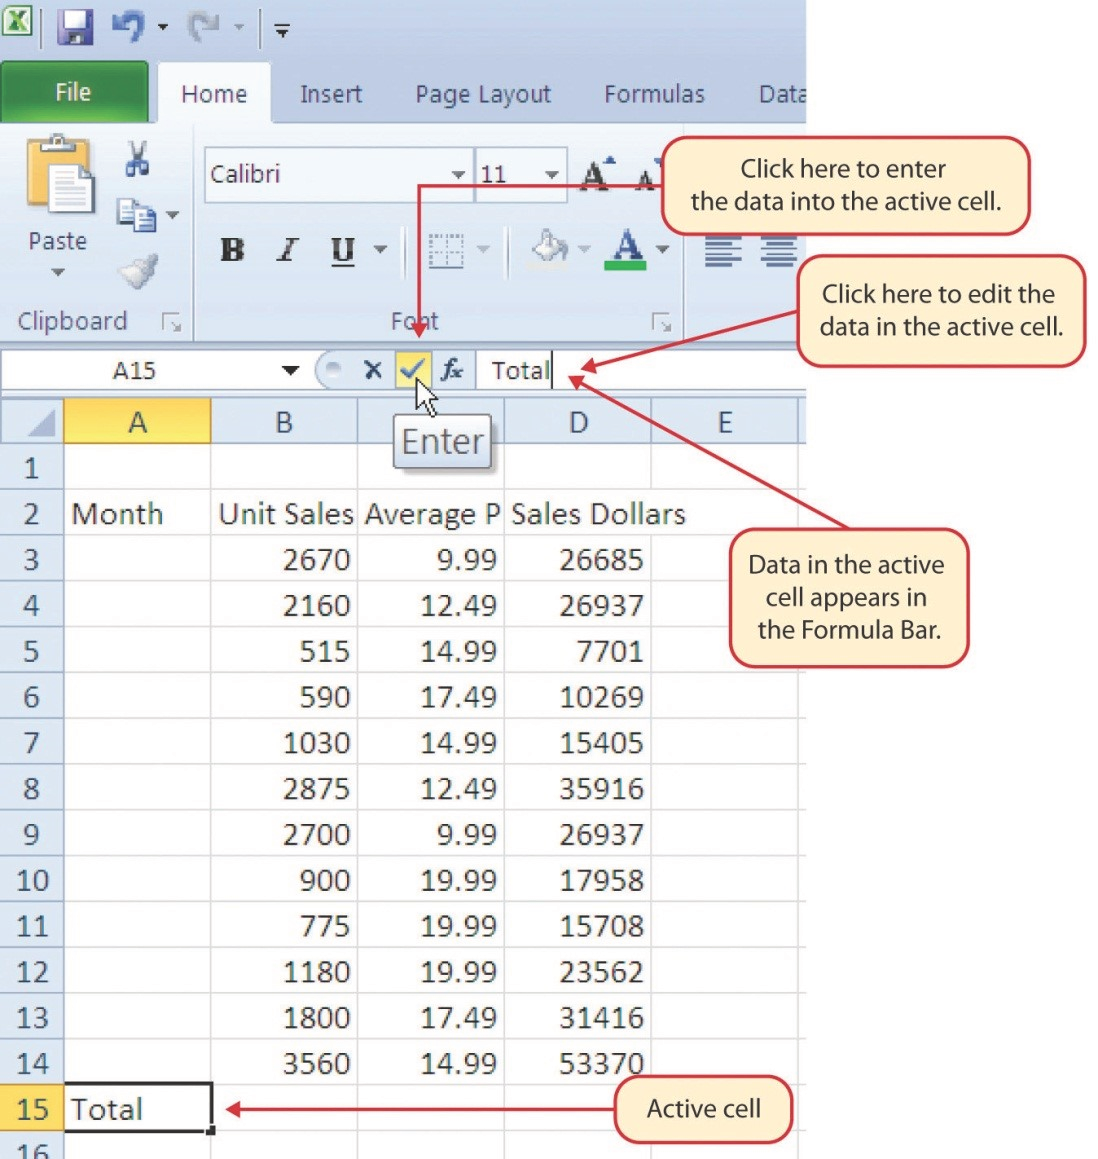
\includegraphics[width=\maxwidth{.95\linewidth}]{gfx/ch01_fig17}
	\caption{Using the Formula Bar to Edit and Enter Data}
	\label{01:fig17}
\end{figure}

\begin{enumerate}[resume]
	\item Double click cell \fmtLoc{A15}.
	\item Add a space after the word \textit{Total} and type the word \fmtTyping{Sales}.
	\item Press the \fmtKeystroke{Enter} key.
\end{enumerate}

\begin{center}
	\begin{shtcutbox}{Keyboard Shortcuts}
		\textbf{Editing Data in a Cell}
		\\
		\begin{itemize}
			\setlength{\itemsep}{0pt}
			\setlength{\parskip}{0pt}
			\setlength{\parsep}{0pt}
			
			\item Click in the cell that is to be edited and press the \fmtKeystroke{F2} key on the keyboard. Alternatively, double-click the cell to be edited.
			
		\end{itemize}
	\end{shtcutbox}
\end{center}

\subsection{Auto Fill}

The \textit{Auto Fill} feature is a valuable tool when manually entering data into a worksheet. This feature has many uses, but it is most beneficial when entering data in a defined sequence, such as the numbers $ 2 $, $ 4 $, $ 6 $, $ 8 $, and so on, or non-numeric data such as the days of the week or months of the year. The following steps demonstrate how the \textit{Auto Fill Handle} can be used to enter the months of the year in \textit{Column A}.

\begin{enumerate}
	\item Click cell \fmtLoc{A3} in the \fmtWorksheet{Sheet1} worksheet.
	\item Type the word \fmtTyping{January} and press the \fmtKeystroke{Enter} key.
	\item Click in cell \fmtLoc{A3} again.
	\item Move the mouse pointer to the lower right corner of cell \fmtLoc{A3}. Notice a small square in this corner of the cell which is called the \fmtButton{Auto Fill Handle} (See Figure \ref{01:fig18}) When the mouse pointer gets close to the \fmtButton{Auto Fill Handle}, the pointer's white block plus sign will turn into a black plus sign.
\end{enumerate}

\begin{figure}[H]
	\centering
	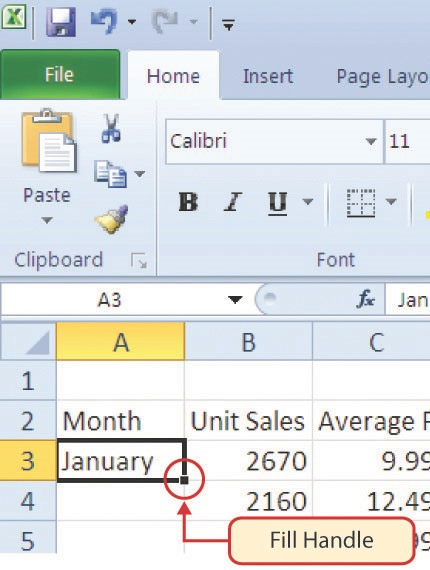
\includegraphics[width=\maxwidth{.95\linewidth}]{gfx/ch01_fig18}
	\caption{Auto Fill Handle}
	\label{01:fig18}
\end{figure}

\begin{enumerate}[resume]
	\item Left click and drag the \fmtButton{Auto Fill Handle} to cell \fmtLoc{A14}. Notice that the \fmtButton{Auto Fill Handle} tip box indicates what month will be placed into each cell (see Figure \ref{01:fig19}). Release the left mouse button when the tip box reads \textit{December}.
\end{enumerate}

\begin{figure}[H]
	\centering
	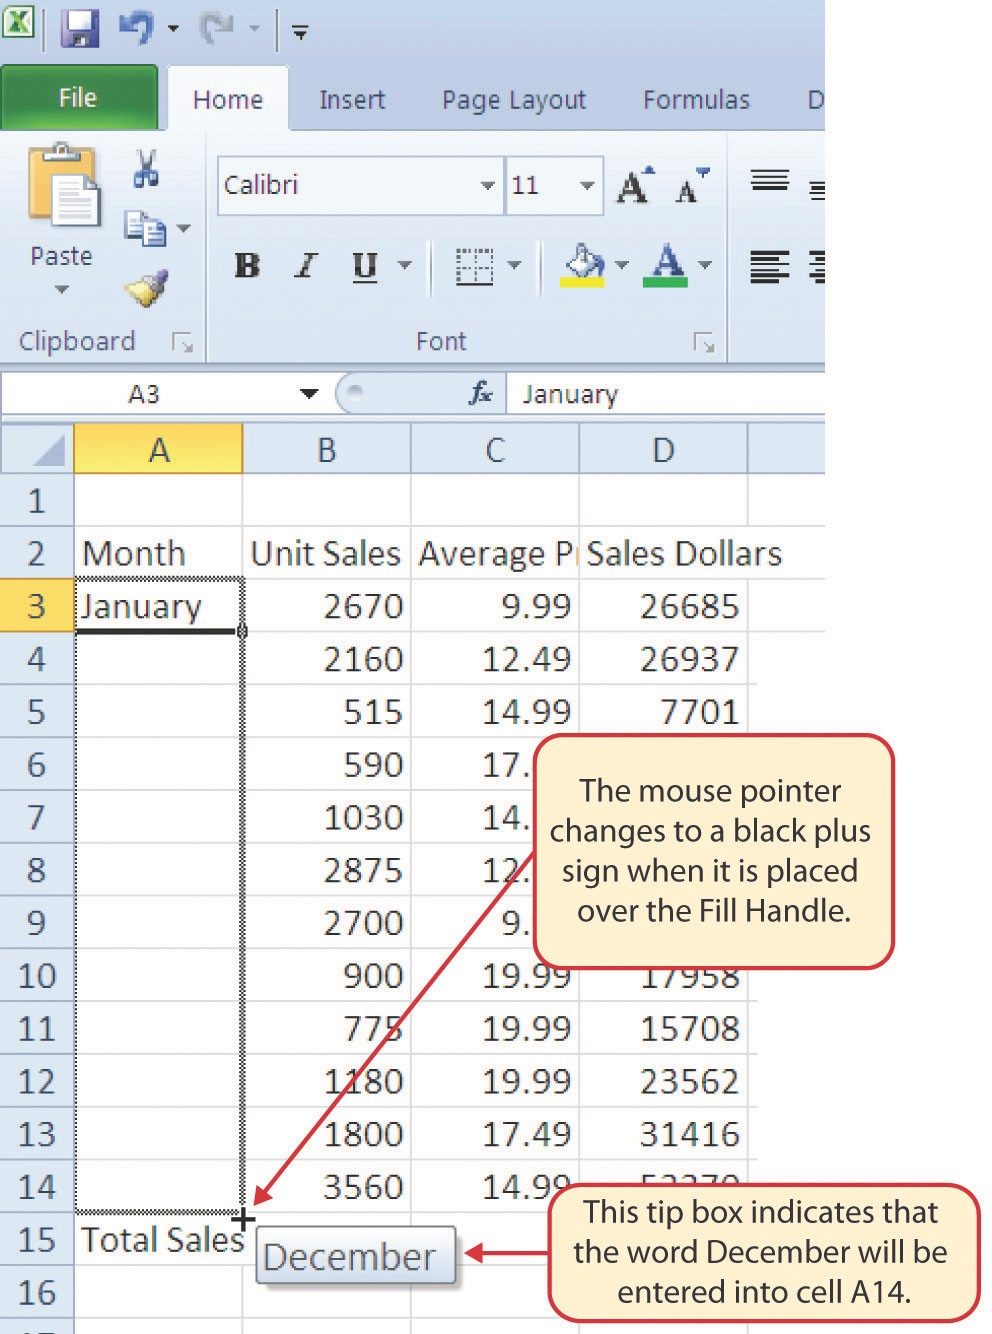
\includegraphics[width=\maxwidth{.95\linewidth}]{gfx/ch01_fig19}
	\caption{Using Auto Fill Handle to Enter the Months of the Year}
	\label{01:fig19}
\end{figure}

Once the left mouse button is released, all twelve months of the year should appear in the cell range $ A3 $:$ A14 $, as shown in Figure \ref{01:fig20}. After auto-filling a range, an \textit{Auto Fill Options} button pops up at the lower left corner of the filled range, as shown in Figure \ref{01:fig20}. 

Excel \fmtOldExcel{2016}. The \textit{Auto Fill Options} button presents several options for changing the way that the range is filled.

\begin{figure}[H]
	\centering
	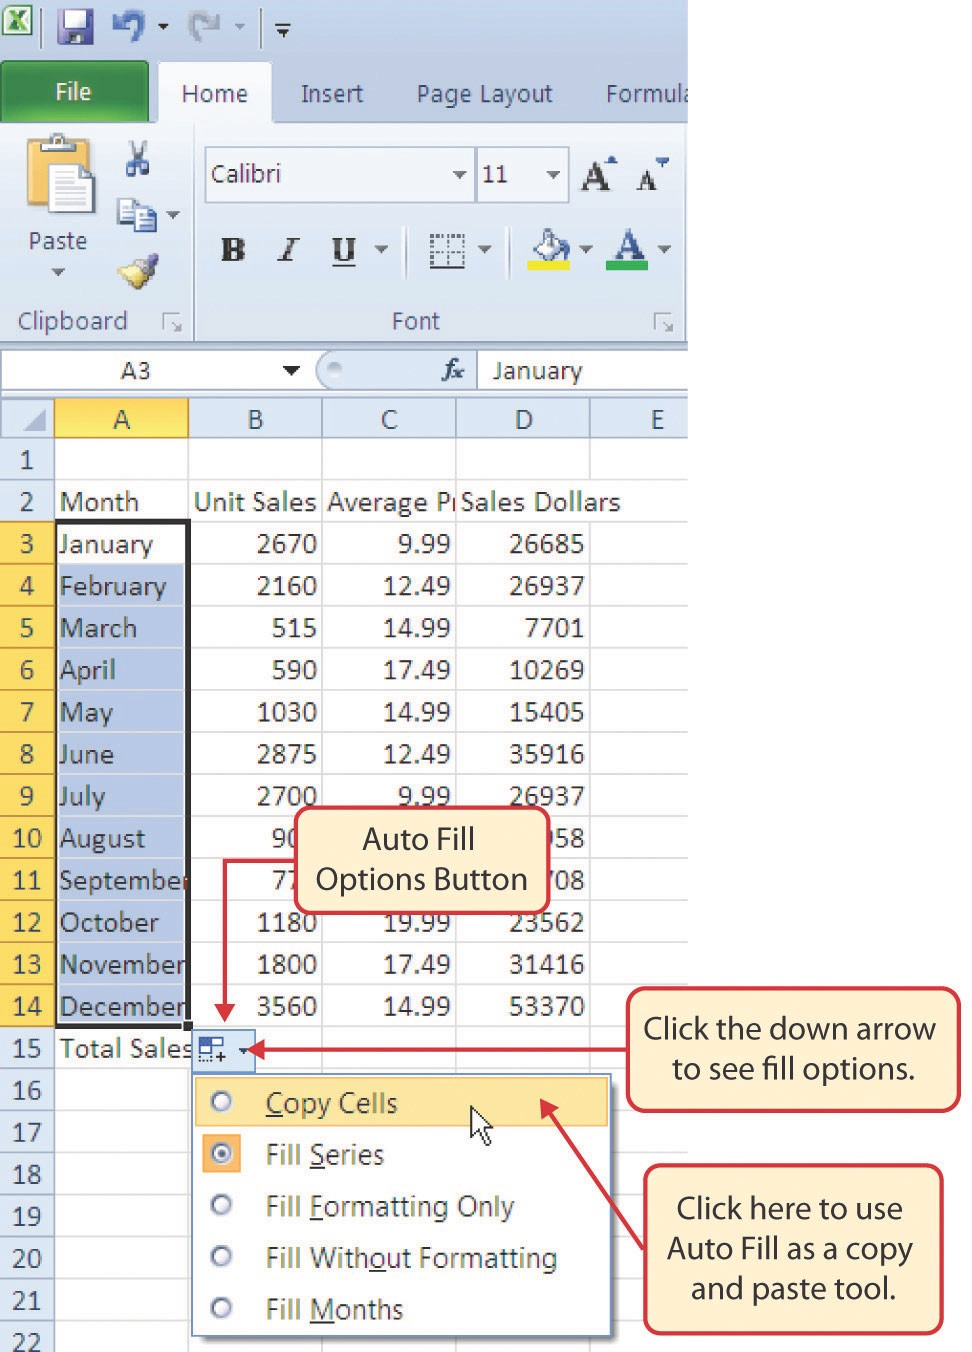
\includegraphics[width=\maxwidth{.95\linewidth}]{gfx/ch01_fig20}
	\caption{Auto Fill Options Button}
	\label{01:fig20}
\end{figure}

\begin{enumerate}
	\item Click the \fmtButton{Auto Fill Options} button.
	\item Click the \fmtButton{Copy Cells} option. This will change the months in the range \fmtLoc{A4:A14} to January.
	\item Click the \fmtButton{Auto Fill Options} button again.
	\item Click the \fmtButton{Fill Months} option to return the months of the year to the cell range \fmtLoc{A4:A14}. The \fmtButton{Fill Series} option will provide the same result.
\end{enumerate}

Excel \fmtNewExcel{365}. The \textit{Auto Fill Options} button was replaced with the \textit{Quick Analysis} button. That button will apply several possible analysis features to the filled range, like highlighting entries that are duplicates.

\begin{figure}[H]
	\centering
	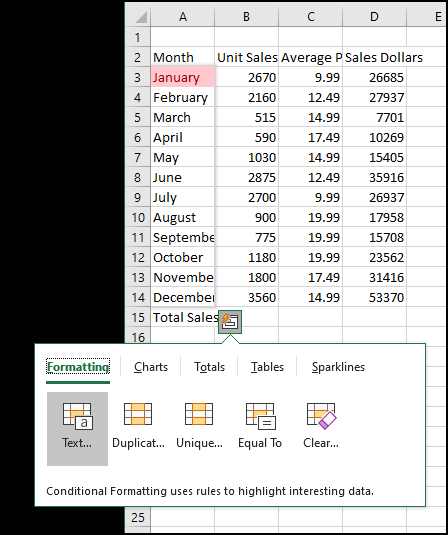
\includegraphics[width=\maxwidth{.95\linewidth}]{gfx/ch01_fig20a}
	\caption{Quick Analysis Button}
	\label{01:fig20a}
\end{figure}

\begin{enumerate}
	\item Click the \fmtButton{Quick Analysis} button.
	\item Hover the mouse over each of the Format tab options and notice how the text in the cells is highlighted.
	\item Click anywhere in the worksheet to finish the auto fill process.
\end{enumerate}

\subsection{Deleting Data and the Undo Command}

There are several methods for removing data from a worksheet, a few of which are demonstrated here. With each method, use the \textit{Undo} command to return the data that was deleted. Undo is available on the Quick Access Toolbar or use the keyboard shortcut of \fmtKeystroke{Ctrl} $ + $ \fmtKeystroke{Z}.This is a helpful command in the event that data is mistakenly deleted from the worksheet. The following steps demonstrate how to delete data from a cell or range of cells.

\begin{enumerate}
	\item Click cell \fmtLoc{C2} by placing the mouse pointer over the cell and clicking the left mouse button.
	\item Press the \fmtKeystroke{Delete} key on the keyboard. This removes the contents of the cell.
	\item Highlight the range \fmtLoc{C3:C14} by placing the mouse pointer over cell \fmtLoc{C3} then left click and drag the mouse pointer down to cell \fmtLoc{C14}.
	\item Place the mouse pointer over the \fmtButton{Auto Fill Handle}. Notice that the white block plus sign change to a black plus sign.
	\item Click and drag the mouse pointer up to cell \fmtLoc{C3}, as in Figure \ref{01:fig21}. Release the mouse button. The contents in the range \fmtLoc{C3:C14} will be removed.
\end{enumerate}

\begin{figure}[H]
	\centering
	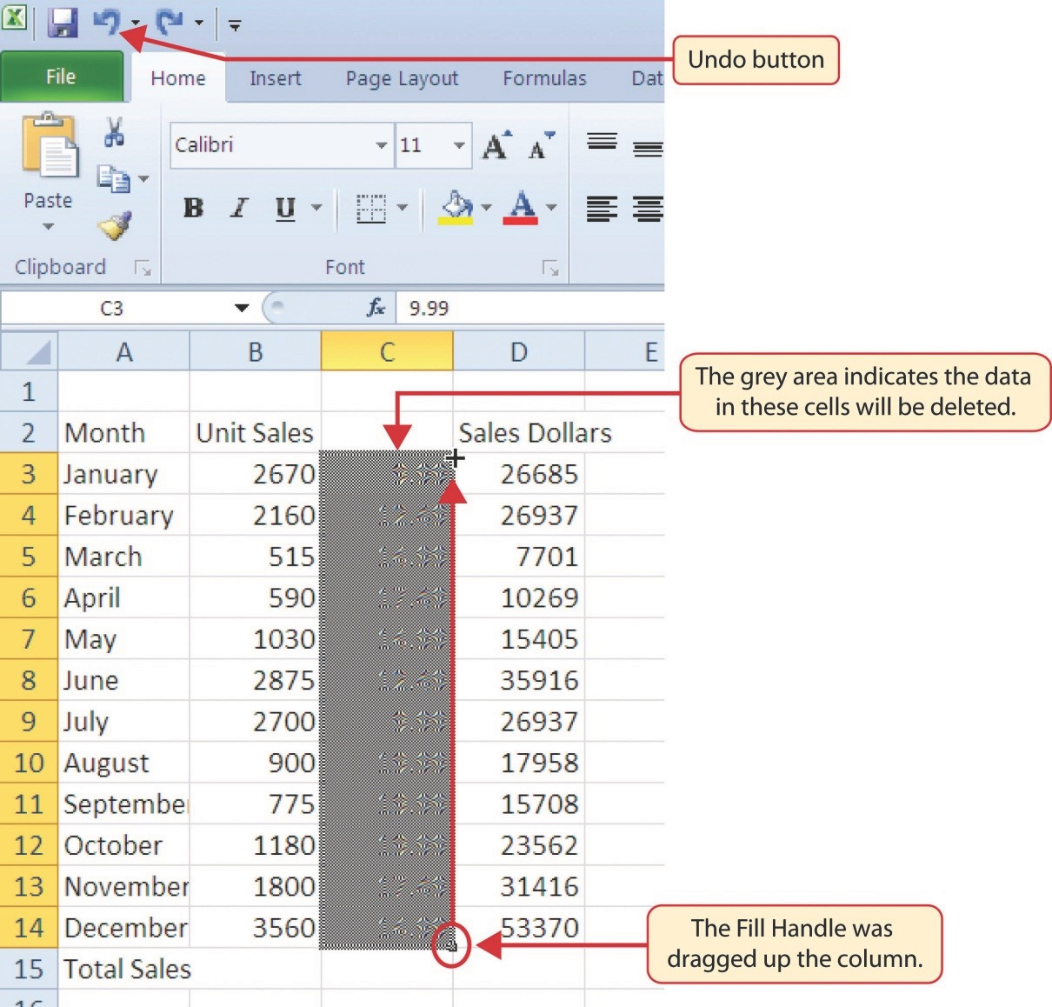
\includegraphics[width=\maxwidth{.95\linewidth}]{gfx/ch01_fig21}
	\caption{Using Auto Fill to Delete Contents of Cell}
	\label{01:fig21}
\end{figure}

\begin{enumerate}
	\item Click the \fmtButton{Undo} button in the \fmtButton{Quick Access Toolbar}, as illustrated in Figure \ref{01:fig21}. This should replace the data in the range \fmtLoc{C3:C14}.
	\item Click the \fmtButton{Undo} button again to replace the data in cell \fmtLoc{C2}.
\end{enumerate}

\begin{center}
	\begin{shtcutbox}{Keyboard Shortcuts}
		\textbf{Undo Command}
		\\
		\begin{itemize}
			\setlength{\itemsep}{0pt}
			\setlength{\parskip}{0pt}
			\setlength{\parsep}{0pt}
			
			\item Hold down the \fmtKeystroke{Ctrl} key while pressing the letter \fmtKeystroke{Z} on the keyboard.
			
		\end{itemize}
	\end{shtcutbox}
\end{center}

\begin{enumerate}[resume]
	\item Highlight the range \fmtLoc{C2:C14} by placing the mouse pointer over cell \fmtLoc{C2}. Then left click and drag the mouse pointer down to cell \fmtLoc{C14}.
	\item Click \fmtButton{Home $ \Rightarrow $ Editing $ \Rightarrow $ Clear} (see Figure \ref{01:fig22}). This opens a drop-down menu that contains several options for removing or clearing data from a cell. Notice that there are also options for clearing just the formats or the hyperlinks in a cell.
	\item Click the \fmtButton{Clear All} option. This removes the data in the cell range.
	\item Click the \fmtButton{Undo} button. This replaces the data in the range \fmtLoc{C2:C14}.
\end{enumerate}

\begin{figure}[H]
	\centering
	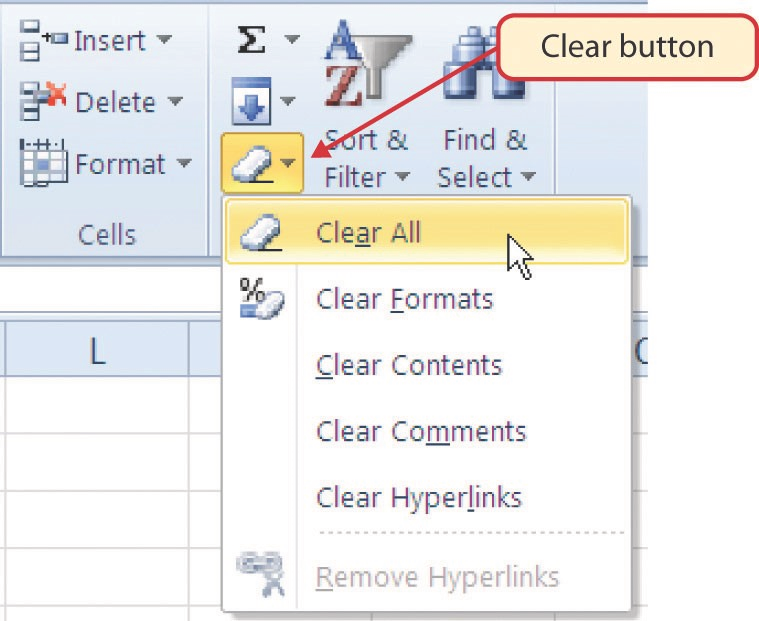
\includegraphics[width=\maxwidth{.95\linewidth}]{gfx/ch01_fig22}
	\caption{Clear Command Drop-Down Menu}
	\label{01:fig22}
\end{figure}

\subsection{Adjusting Columns and Rows}

There are a few entries in the worksheet that appear to be cut off. For example, the last letter of the word \textit{September} cannot be seen in cell $ A11 $. This is because the column is too narrow for this word. The columns and rows on an Excel worksheet can be adjusted to accommodate the data that is being entered into a cell. The following steps explain how to adjust the column widths and row heights in a worksheet.

\begin{enumerate}
	\item Bring the mouse pointer between \fmtLoc{Column A} and \fmtLoc{Column B} in the \fmtWorksheet{Sheet1} worksheet, as shown in Figure \ref{01:fig23}. Notice that the pointer's white block plus sign turns into double arrows.
	\item Click and drag the column to the right so the entire word \textit{September} in cell \fmtLoc{A11} can be seen. As the column separator is dragged to the right the column width pops up in a tip box. This box displays the number of characters that will fit into the column using the Calibri 11-point font which is the default setting for font/size.
	\item Release the left mouse button.
\end{enumerate}

\begin{figure}[H]
	\centering
	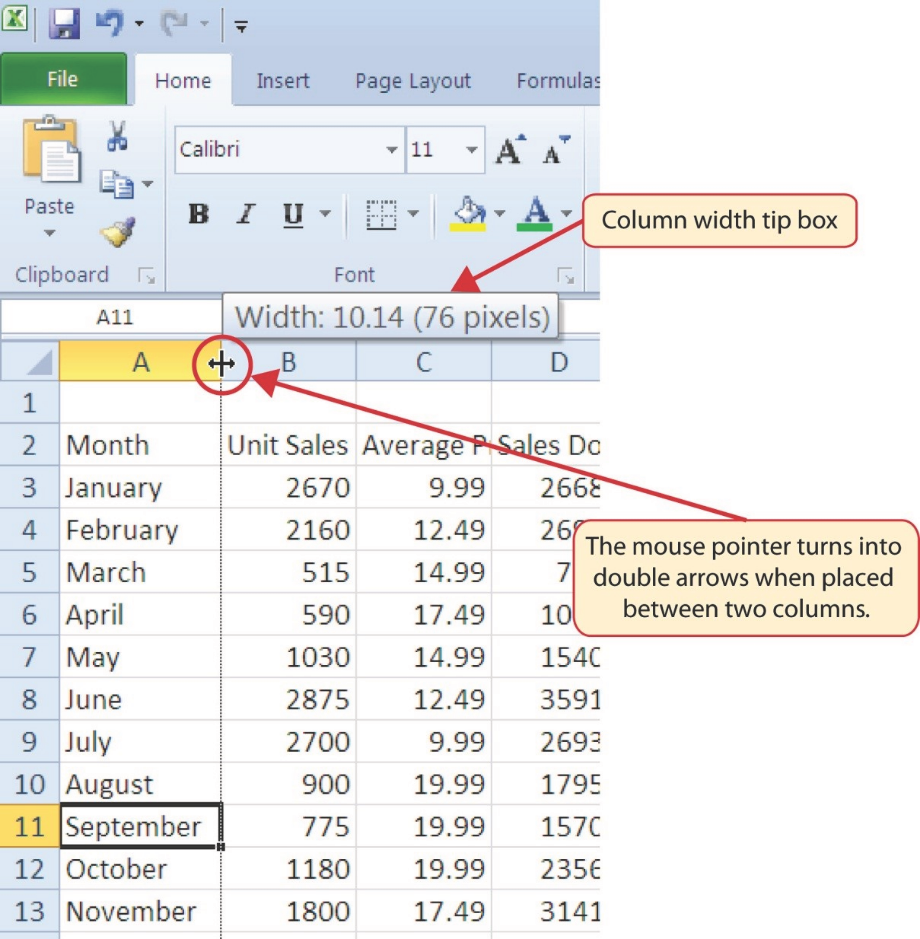
\includegraphics[width=\maxwidth{.95\linewidth}]{gfx/ch01_fig23}
	\caption{Adjusting Column Widths}
	\label{01:fig23}
\end{figure}

The click-and-drag method can be inefficient to set a specific character width for more than one column. The following steps illustrate a second method for adjusting columns to a specific width.

\begin{enumerate}
	\item Click any cell location in \fmtLoc{Column A} by moving the mouse pointer over a cell location and clicking the left mouse button. 
	\item Click \fmtButton{Home $ \Rightarrow $ Cells $ \Rightarrow $ Format $ \Rightarrow $ Column Width}. This will open the \textit{Column Width} dialog box.
	\item Type the number \fmtTyping{13} and click the \fmtButton{OK} button on the \textit{Column Width} dialog box. This will set \fmtLoc{Column A} to this character width (see Figure \ref{01:fig24}).
	\item As a third option, bring the mouse pointer between \fmtLoc{Column A} and \fmtLoc{Column B} so that the double arrow pointer displays and then double-click. This activates \fmtButton{AutoFit}, which adjusts the column width based on the longest entry in the column.
	\item Use the \textit{Column Width} dialog box to set the width to \fmtTyping{13}.
\end{enumerate}

\begin{figure}[H]
	\centering
	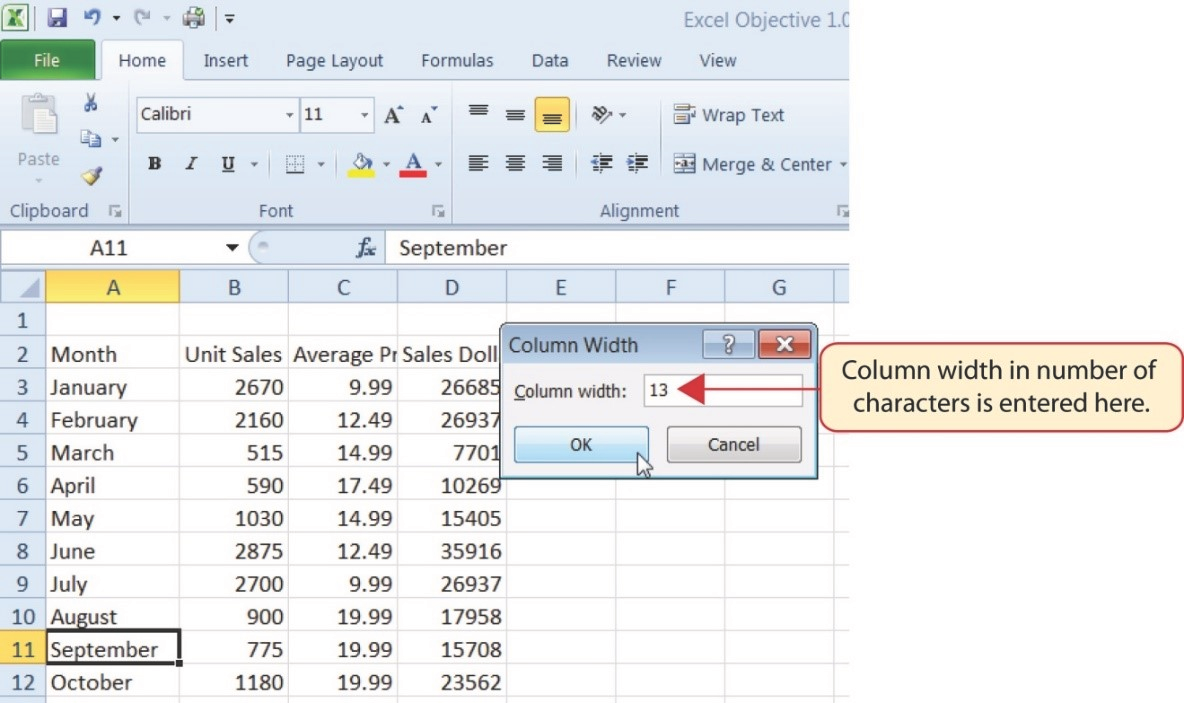
\includegraphics[width=\maxwidth{.95\linewidth}]{gfx/ch01_fig24}
	\caption{Column Width Dialog Box}
	\label{01:fig24}
\end{figure}

\begin{center}
	\begin{shtcutbox}{Keyboard Shortcuts}
		\textbf{Column Width}
		\\
		\begin{itemize}
			\setlength{\itemsep}{0pt}
			\setlength{\parskip}{0pt}
			\setlength{\parsep}{0pt}
			
			\item Press and release the \fmtKeystroke{Alt} key on the keyboard and then press the letters \fmtKeystroke{H}, \fmtKeystroke{O}, and \fmtKeystroke{W} one at a time.
			
		\end{itemize}
	\end{shtcutbox}
\end{center}

The following steps demonstrate how to adjust row height, which is similar to adjusting column width.

\begin{enumerate}
	\item Click cell \fmtLoc{A15}.
	\item Click \fmtButton{Home $ \Rightarrow $ Cells $ \Rightarrow $ Format $ \Rightarrow $ Row Height}. This will open the \textit{Row Height} dialog box.
	\item Type the number \fmtTyping{24} and click the \fmtButton{OK} button on the \textit{Row Height} dialog box. This will set \fmtLoc{Row $ 15 $} to a height of $ 24 $ points. A point is equivalent to approximately $ 1/72 $ of an inch. This adjustment in row height was made to create space between the totals for this worksheet and the rest of the data.
	\item Row height can also be adjusted by dragging the border between \fmtLoc{Row 15} and \fmtLoc{Row 16} or by double-clicking the border between \fmtLoc{Row 15} and \fmtLoc{Row 16}.
\end{enumerate}

\begin{center}
	\begin{shtcutbox}{Keyboard Shortcuts}
		\textbf{Column Width}
		\\
		\begin{itemize}
			\setlength{\itemsep}{0pt}
			\setlength{\parskip}{0pt}
			\setlength{\parsep}{0pt}
			
			\item Press the \fmtKeystroke{Alt} key on the keyboard, then press the letters \fmtKeystroke{H}, \fmtKeystroke{O}, and \fmtKeystroke{H} one at a time.
			
		\end{itemize}
	\end{shtcutbox}
\end{center}

Figure \ref{01:fig25} shows the appearance of the worksheet after \fmtLoc{Column A} and \fmtLoc{Row $ 15 $} are adjusted.

\begin{figure}[H]
	\centering
	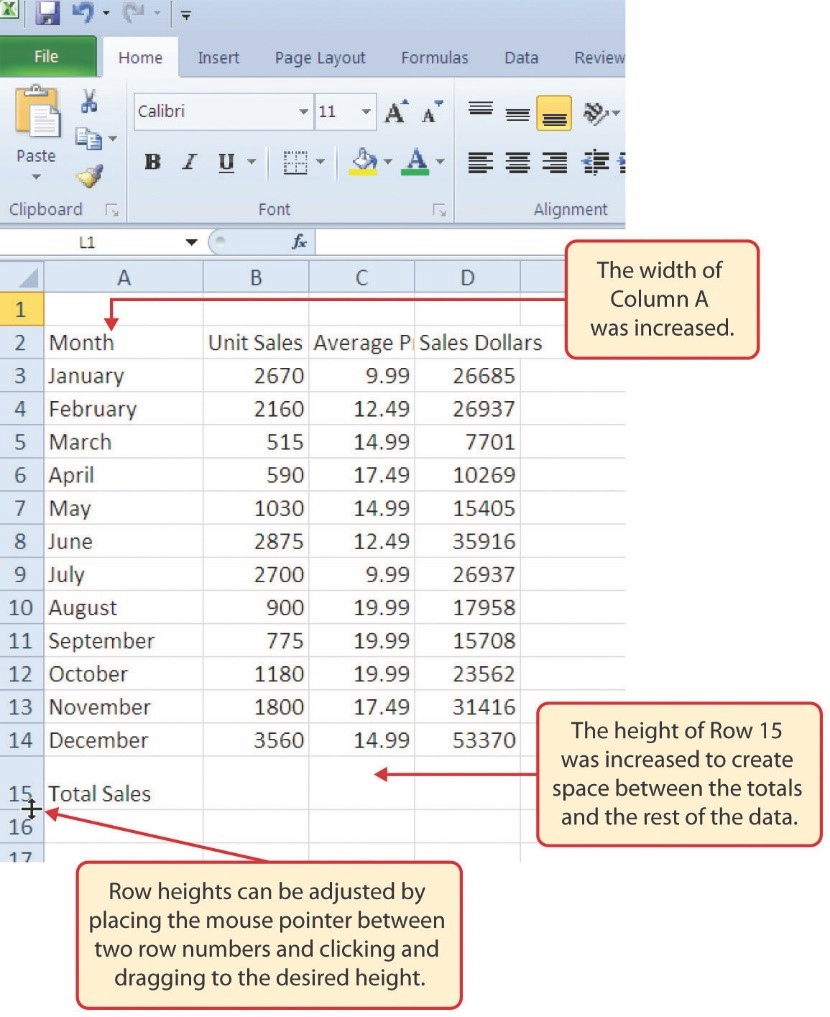
\includegraphics[width=\maxwidth{.95\linewidth}]{gfx/ch01_fig25}
	\caption{CH1-GMW Sales Data with Column A and Row 15 Adjusted}
	\label{01:fig25}
\end{figure}

\begin{center}
	\begin{sklbox}{Skill Refresher}
		\textbf{Adjusting Columns and Rows}
		\\
		\begin{itemize}
			\setlength{\itemsep}{0pt}
			\setlength{\parskip}{0pt}
			\setlength{\parsep}{0pt}
			
			\item Activate at least one cell in the row or column being adjusted.
			\item Click \fmtButton{Home $ \Rightarrow $ Cells $ \Rightarrow $ Format}
			\item Click either \fmtButton{Row Height} or \fmtButton{Column Width} from the drop-down menu.
			\item Enter the Row Height in points or Column Width in characters in the dialog box.
			\item Click the \fmtButton{OK} button.
			
		\end{itemize}
	\end{sklbox}
\end{center}

\subsection{Hiding Columns and Rows}

In addition to adjusting the columns and rows on a worksheet, they can also be hidden. This is a useful technique for enhancing the visual appearance of a worksheet that contains data that is not necessary to display. These features will be demonstrated using the \textit{CH1-GMW Sales Data} workbook later in the course; however, there is no need to have hidden columns or rows in this worksheet. The use of these skills will be presented here for demonstration purposes only.

\begin{enumerate}
	\item Click cell \fmtLoc{C1} in the \fmtWorksheet{Sheet1} worksheet.
	\item Click \fmtButton{Home $ \Rightarrow $ Cells $ \Rightarrow $ Format $ \Rightarrow $ Hide \& Unhide}. This will open a submenu of options.
	\item Click the \fmtButton{Hide Columns} option in the submenu of options (see Figure \ref{01:fig26}) to hide \fmtLoc{Column C}.
\end{enumerate}

\begin{figure}[H]
	\centering
	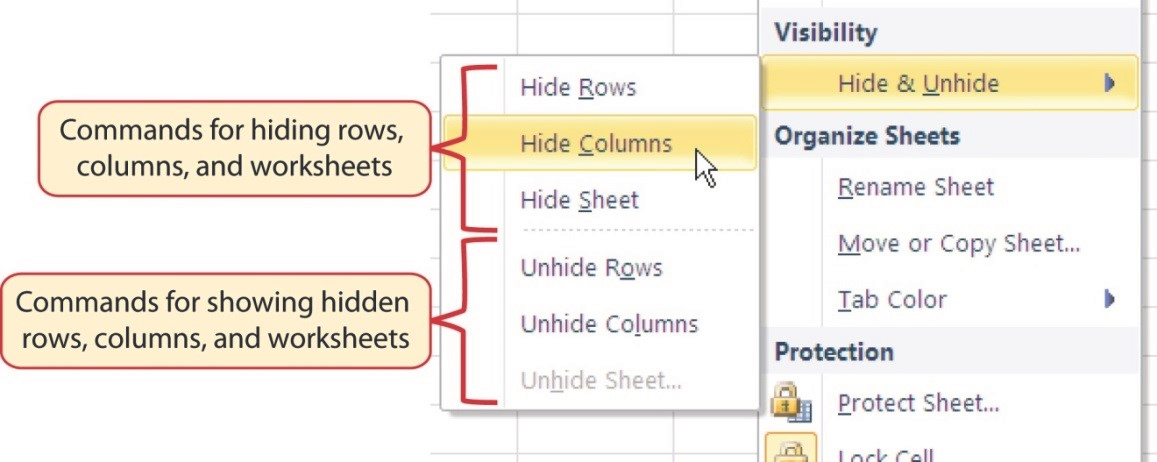
\includegraphics[width=\maxwidth{.95\linewidth}]{gfx/ch01_fig26}
	\caption{Hide \& Unhide Submenu}
	\label{01:fig26}
\end{figure}

\begin{center}
	\begin{shtcutbox}{Keyboard Shortcuts}
		\textbf{Hiding Columns}
		\\
		\begin{itemize}
			\setlength{\itemsep}{0pt}
			\setlength{\parskip}{0pt}
			\setlength{\parsep}{0pt}
			
			\item Hold down the \fmtKeystroke{Ctrl} key while pressing the number \fmtKeystroke{0} on the keyboard. (Note, this is the number zero, not the letter O.)
			
		\end{itemize}
	\end{shtcutbox}
\end{center}

Figure \ref{01:fig27} shows the workbook with \textit{Column C} hidden. If a column is hidden, its name is missing, like the missing letter \textit{C} at the top of the column.

\begin{figure}[H]
	\centering
	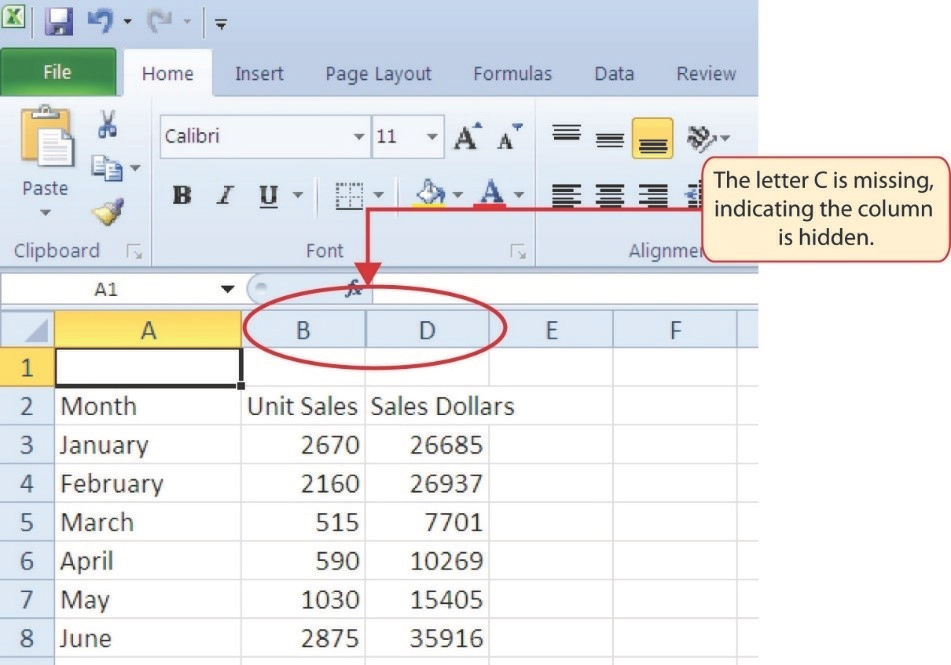
\includegraphics[width=\maxwidth{.95\linewidth}]{gfx/ch01_fig27}
	\caption{Hidden Column}
	\label{01:fig27}
\end{figure}

To unhide a column, use the following steps.

\begin{enumerate}
	\item Highlight the range \fmtLoc{B1:D1} by activating cell \fmtLoc{B1} and clicking and dragging over to cell \fmtLoc{D1}.
	\item Click \fmtButton{Home $ \Rightarrow $ Cells $ \Rightarrow $ Format $ \Rightarrow $ Hide \& Unhide}. 
	\item Click the \fmtButton{Unhide Columns} option in the submenu of options. \fmtLoc{Column C} will now be visible on the worksheet.
\end{enumerate}

\begin{center}
	\begin{shtcutbox}{Keyboard Shortcuts}
		\textbf{Unhiding Columns}
		\\
		\begin{itemize}
			\setlength{\itemsep}{0pt}
			\setlength{\parskip}{0pt}
			\setlength{\parsep}{0pt}
			
			\item Highlight cells on either side of the hidden column(s), then hold down the \fmtKeystroke{Ctrl} key and the \fmtKeystroke{Shift} key while pressing \fmtKeystroke{)}, the close parenthesis key, on the keyboard. Note: This keyboard shortcut does not reliably work for some reason that has not been explained by Microsoft. If it does not work, then use the ribbon button.
			
		\end{itemize}
	\end{shtcutbox}
\end{center}

The following steps demonstrate how to hide rows, which is similar to hiding columns.

\begin{enumerate}
	\item Click cell \fmtLoc{A3} in the \fmtWorksheet{Sheet1} worksheet.
	\item Click \fmtButton{Home $ \Rightarrow $ Cells $ \Rightarrow $ Format $ \Rightarrow $ Hide \& Unhide}. This will open a submenu of options.
	\item Click the \fmtButton{Hide Rows} option in the submenu of options. This will hide \fmtLoc{Row 3}.
\end{enumerate}

\begin{center}
	\begin{shtcutbox}{Keyboard Shortcuts}
		\textbf{Hiding Rows}
		\\
		\begin{itemize}
			\setlength{\itemsep}{0pt}
			\setlength{\parskip}{0pt}
			\setlength{\parsep}{0pt}
			
			\item Hold down the \fmtKeystroke{Ctrl} key while pressing the number \fmtKeystroke{9} key on the keyboard.
			
		\end{itemize}
	\end{shtcutbox}
\end{center}

To unhide a row, follow these steps.

\begin{enumerate}
	\item Highlight the range \fmtLoc{A2:A4} by activating cell \fmtLoc{A2} and clicking and dragging over to cell \fmtLoc{A4}.
	\item Click \fmtButton{Home $ \Rightarrow $ Cells $ \Rightarrow $ Format $ \Rightarrow $ Hide \& Unhide}. This will open a submenu of options.
	\item Click the \fmtButton{Unhide Rows} option in the submenu of options to unhide \fmtLoc{Row 3}.
\end{enumerate}

\begin{center}
	\begin{shtcutbox}{Keyboard Shortcuts}
		\textbf{Unhiding Rows}
		\\
		\begin{itemize}
			\setlength{\itemsep}{0pt}
			\setlength{\parskip}{0pt}
			\setlength{\parsep}{0pt}
			
			\item Highlight cells above and below the hidden row(s), then hold down the \fmtKeystroke{Ctrl} key and the \fmtKeystroke{Shift} key while pressing \fmtKeystroke{(}, the open parenthesis key, on the keyboard.
			
		\end{itemize}
	\end{shtcutbox}
\end{center}

\begin{center}
	\begin{sklbox}{Skill Refresher}
		\textbf{Hiding Columns and Rows}
		\\
		\begin{itemize}
			\setlength{\itemsep}{0pt}
			\setlength{\parskip}{0pt}
			\setlength{\parsep}{0pt}
			
			\item Activate at least one cell in the row(s) or column(s) being hidden.
			\item Click \fmtButton{Home $ \Rightarrow $ Cells $ \Rightarrow $ Format $ \Rightarrow $ Hide \& Unhide}
			\item Click either the \fmtButton{Hide Rows} or \fmtButton{Hide Columns} option.
			
		\end{itemize}
	\end{sklbox}
\end{center}


\begin{center}
	\begin{sklbox}{Skill Refresher}
		\textbf{Unhiding Columns and Rows}
		\\
		\begin{itemize}
			\setlength{\itemsep}{0pt}
			\setlength{\parskip}{0pt}
			\setlength{\parsep}{0pt}
			
			\item Highlight the cells above and below the hidden row(s) or to the left and right of the hidden column(s).
			\item Click \fmtButton{Home $ \Rightarrow $ Cells $ \Rightarrow $ Format $ \Rightarrow $ Hide \& Unhide}
			\item Click either the \fmtButton{Unhide Rows} or \fmtButton{Unhide Columns} option.
			
		\end{itemize}
	\end{sklbox}
\end{center}

\begin{center}
	\begin{infobox}{Integrity Check}
		\textbf{Hidden Rows and Columns}
		\\
		\\
		In most careers, it is common for professionals to use Excel workbooks that have been designed by a coworker. Before using a workbook developed by someone else, always check for hidden rows and columns. It is easy to determine if a row or column is hidden by looking for missing row  numbers or column letters.
	\end{infobox}
\end{center}

\subsection{Inserting Columns and Rows}

Using Excel workbooks that have been created by others is a very efficient way to work because it eliminates the need to create worksheets from scratch. However, to accomplish a specific goal, additional columns or rows may need to be added to a worksheet. In this case, blank columns or rows are inserted into a worksheet as demonstrated below.

\begin{enumerate}
	\item Click cell \fmtLoc{C1} in the \fmtWorksheet{Sheet1} worksheet.
	\item Click \fmtButton{Home $ \Rightarrow $ Cells $ \Rightarrow $ Insert $ \Rightarrow $ Down Arrow} (see Figure \ref{01:fig28}).
\end{enumerate}

\begin{figure}[H]
	\centering
	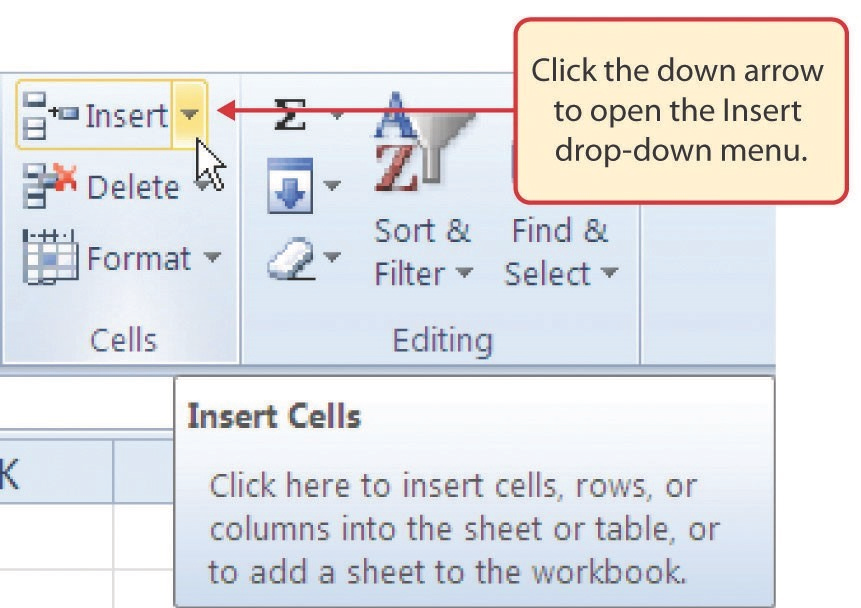
\includegraphics[width=\maxwidth{.95\linewidth}]{gfx/ch01_fig28}
	\caption{Insert Button (Down Arrow)}
	\label{01:fig28}
\end{figure}

\begin{enumerate}[resume]
	\item Click the \fmtButton{Insert Sheet Columns} option from the drop-down menu (see Figure \ref{01:fig29}). A blank column will be inserted to the left of \fmtLoc{Column C}. The contents that were previously in \fmtLoc{Column C} now appear in \fmtLoc{Column D}. Note that columns are always inserted to the left of the activated cell.

\end{enumerate}

\begin{figure}[H]
	\centering
	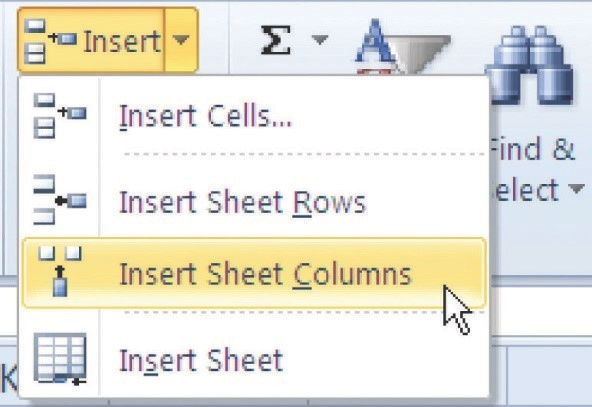
\includegraphics[width=\maxwidth{.95\linewidth}]{gfx/ch01_fig29}
	\caption{Insert Drop-Down Menu}
	\label{01:fig29}
\end{figure}

\begin{center}
	\begin{shtcutbox}{Keyboard Shortcuts}
		\textbf{Inserting Columns}
		\\
		\begin{itemize}
			\setlength{\itemsep}{0pt}
			\setlength{\parskip}{0pt}
			\setlength{\parsep}{0pt}
			
			\item Press the \fmtKeystroke{Alt} key and then the letters \fmtKeystroke{H}, \fmtKeystroke{I}, and \fmtKeystroke{C} one at a time. A column will be inserted to the left of the activated cell.
			
		\end{itemize}
	\end{shtcutbox}
\end{center}

\begin{enumerate}[resume]
	\item Click cell \fmtLoc{A3} in the \fmtWorksheet{Sheet1} worksheet.
	\item Click \fmtButton{Home $ \Rightarrow $ Cells $ \Rightarrow $ Insert $ \Rightarrow $ Down Arrow} (see Figure \ref{01:fig28}).
	\item Click the \fmtButton{Insert Sheet Rows} option from the drop-down menu (see Figure \ref{01:fig29}). A blank row will be inserted above \fmtLoc{Row $ 3 $}. The contents that were previously in \fmtLoc{Row $ 3 $} now appear in \fmtLoc{Row $ 4 $}. Note that rows are always inserted above the activated cell.
\end{enumerate}

\begin{center}
	\begin{shtcutbox}{Keyboard Shortcuts}
		\textbf{Inserting Rpws}
		\\
		\begin{itemize}
			\setlength{\itemsep}{0pt}
			\setlength{\parskip}{0pt}
			\setlength{\parsep}{0pt}
			
			\item Press the \fmtKeystroke{Alt} key and then the letters \fmtKeystroke{H}, \fmtKeystroke{I}, and \fmtKeystroke{R} one at a time. A row will be inserted above the activated cell.
			
		\end{itemize}
	\end{shtcutbox}
\end{center}

\begin{center}
	\begin{sklbox}{Skill Refresher}
		\textbf{Inserting Columns and Rows}
		\\
		\begin{itemize}
			\setlength{\itemsep}{0pt}
			\setlength{\parskip}{0pt}
			\setlength{\parsep}{0pt}
			
			\item Activate the cell to the right of the desired blank column or below the desired blank row.
			\item Click \fmtButton{Home $ \Rightarrow $ Cells $ \Rightarrow $ Insert $ \Rightarrow $ Down Arrow}
			\item Click either the \fmtButton{Insert Sheet Columns} or \fmtButton{Insert Sheet Rows} option.
			
		\end{itemize}
	\end{sklbox}
\end{center}

\subsection{Moving Data}

Once data is entered into a worksheet, it can be moved to different locations, as demonstrated below.

\begin{enumerate}
	\item Highlight the range \fmtLoc{D2:D15} by clicking cell \fmtLoc{D2} and dragging down to cell \fmtLoc{D15}.
	\item Bring the mouse pointer to the left edge of cell \fmtLoc{D2}. Notice that the white block plus sign change to cross arrows (see Figure \ref{01:fig30}). This indicates that the data can be dragged to a new location by left-clicking the mouse.
\end{enumerate}

\begin{figure}[H]
	\centering
	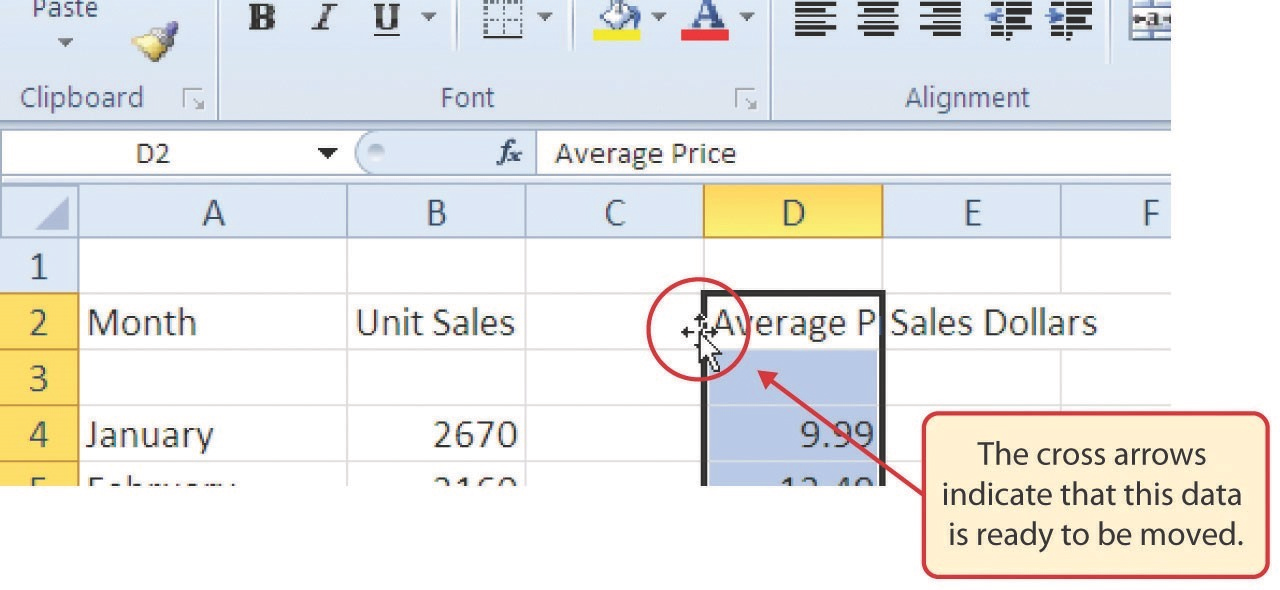
\includegraphics[width=\maxwidth{.95\linewidth}]{gfx/ch01_fig30}
	\caption{Moving Data}
	\label{01:fig30}
\end{figure}

\begin{enumerate}[resume]
	\item Left Click and drag the mouse pointer to cell \fmtLoc{C2}.
	\item Release the left mouse button. The data now appears in \fmtLoc{Column C}.
	\item Click the \textit{Undo} button in the \fmtButton{Quick Access Toolbar}. This moves the data back to \fmtLoc{Column D}.
\end{enumerate}

\begin{center}
	\begin{infobox}{Integrity Check}
		\textbf{Moving Data}
		\\
		\\
		Before moving data on a worksheet, make sure to identify all the components that belong with the series being moved. For example, if a column of data is being moved make sure the column heading is included. Also, make sure all values are highlighted in the column before moving it.
	\end{infobox}
\end{center}


\subsection{Deleting Columns and Rows}

It may occasionally be necessary to delete entire columns or rows of data from a worksheet. For example, a worksheet may contain blank columns or rows that need to be removed. The methods for removing cell contents were covered earlier and can be used to delete unwanted data. However, to delete an entire column or row in a workbook, use the following steps.

\begin{enumerate}
	\item Click cell \fmtLoc{A3}.
	\item Click \fmtButton{Home $ \Rightarrow $ Cells $ \Rightarrow $ Delete $ \Rightarrow $ Down Arrow}
	\item Click the \fmtButton{Delete Sheet Rows} option from the drop-down menu (see Figure \ref{01:fig31}). This removes \fmtLoc{Row 3} and shifts all the data in the worksheet up one row.
\end{enumerate}

\begin{figure}[H]
	\centering
	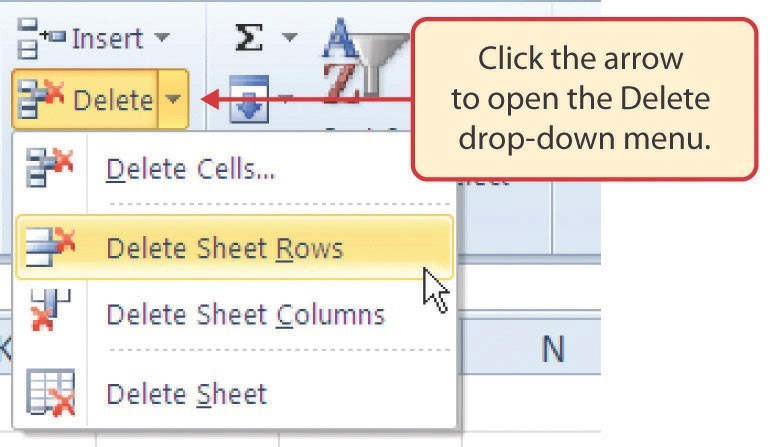
\includegraphics[width=\maxwidth{.95\linewidth}]{gfx/ch01_fig31}
	\caption{Delete Drop-Down Menu}
	\label{01:fig31}
\end{figure}

\begin{center}
	\begin{shtcutbox}{Keyboard Shortcuts}
		\textbf{Deleting Rows}
		\\
		\begin{itemize}
			\setlength{\itemsep}{0pt}
			\setlength{\parskip}{0pt}
			\setlength{\parsep}{0pt}
			
			\item Press the \fmtKeystroke{Alt} key and then the letters \fmtKeystroke{H}, \fmtKeystroke{D}, and \fmtKeystroke{R} one at a time. The row with the activated cell will be deleted.
			
		\end{itemize}
	\end{shtcutbox}
\end{center}

\begin{enumerate}[resume]
	\item Click cell \fmtLoc{C1}.
	\item Click \fmtButton{Home $ \Rightarrow $ Cells $ \Rightarrow $ Delete $ \Rightarrow $ Down Arrow}.
	\item Click the \fmtButton{Delete Sheet Columns} option from the drop-down menu (see Figure \ref{01:fig31}). This removes \fmtLoc{Column C} and shifts all the data in the worksheet over one column to the left.
	\item Save the changes to the workbook by clicking either \fmtButton{Quick Access Toolbar $ \Rightarrow $ Save} or \fmtButton{File $ \Rightarrow $ Save}.
\end{enumerate}

\begin{center}
	\begin{shtcutbox}{Keyboard Shortcuts}
		\textbf{Deleting Columns}
		\\
		\begin{itemize}
			\setlength{\itemsep}{0pt}
			\setlength{\parskip}{0pt}
			\setlength{\parsep}{0pt}
			
			\item Press the \fmtKeystroke{Alt} key and then the letters \fmtKeystroke{H}, \fmtKeystroke{D}, and \fmtKeystroke{C} one at a time. The column with the activated cell will be deleted.
			
		\end{itemize}
	\end{shtcutbox}
\end{center}

\begin{center}
	\begin{sklbox}{Skill Refresher}
		\textbf{Deleting Columns and Rows}
		\\
		\begin{itemize}
			\setlength{\itemsep}{0pt}
			\setlength{\parskip}{0pt}
			\setlength{\parsep}{0pt}
			
			\item Activate any cell in the row or column that is to be deleted.
			\item Click \fmtButton{Home $ \Rightarrow $ Cells $ \Rightarrow $ Delete $ \Rightarrow $ Down Arrow}.
			\item Click either \fmtButton{Delete Sheet Columns} or \fmtButton{Delete Sheet Rows}.
			
		\end{itemize}
	\end{sklbox}
\end{center}

\begin{center}
	\begin{tkwbox}{Key Take-Aways}
		\textbf{Entering, Editing, and Managing Data}
		\\
		\begin{itemize}
			\setlength{\itemsep}{0pt}
			\setlength{\parskip}{0pt}
			\setlength{\parsep}{0pt}
			
			\item Column headings should be used in a worksheet and should accurately describe the data contained in each column.
			\item Using symbols such as dollar signs when entering numbers into a worksheet can slow down the data entry process.
			\item Worksheets must be carefully proofread when data has been manually entered.
			\item The Undo command is a valuable tool for recovering data that was deleted from a worksheet.
			\item When using a worksheet that was developed by someone else, look carefully for hidden columns or rows.
			
		\end{itemize}
	\end{tkwbox}
\end{center}

\section{Formatting and Data Analysis}

\begin{center}
	\begin{objbox}{Learning Objectives}
		\begin{itemize}
			\setlength{\itemsep}{0pt}
			\setlength{\parskip}{0pt}
			\setlength{\parsep}{0pt}
			
			\item Use formatting techniques as introduced in the \textit{Excel Spreadsheet Guidelines}, below, to enhance the appearance of a worksheet.
			\item Understand how to align data in cell locations.
			\item Examine how to enter multiple lines of text in a cell location.
			\item Understand how to add borders to a worksheet.
			\item Examine how to use the AutoSum feature to calculate totals.
			\item Use the Cut, Copy, and Paste commands to manipulate the data on a worksheet.
			\item Understand how to move, rename, insert, and delete worksheet tabs.
		\end{itemize}
	\end{objbox}
\end{center}

This section addresses formatting commands that can be used to enhance the visual appearance of a worksheet. It also provides an introduction to mathematical calculations. The skills introduced in this section provides powerful tools for analyzing the data used in this workbook and will highlight how Excel is used to make key decisions in virtually any career. Additionally, \textit{Excel Spreadsheet Guidelines} for format and appearance will be introduced as a format to be used for the spreadsheets submitted as part of this course.

\subsection{Formatting Data and Cells}

Enhancing the visual appearance of a worksheet is a critical step in creating a valuable tool for coworkers when making key decisions. For example, there are accepted professional formatting standards used when spreadsheets contain only currency data. For this course, the following \textit{Excel Guidelines for Formatting} will be used. Figure \ref{01:fig32} displays how to use Accounting number format when ALL figures are currency. Only the first row of data and the totals should be formatted with the \textit{accounting} format while the other data should be formatted with \textit{comma} style. There also needs to be a top border above the numbers in the total row. If any of the numbers have cents, format all of the data with two decimal places.

\begin{figure}[H]
	\centering
	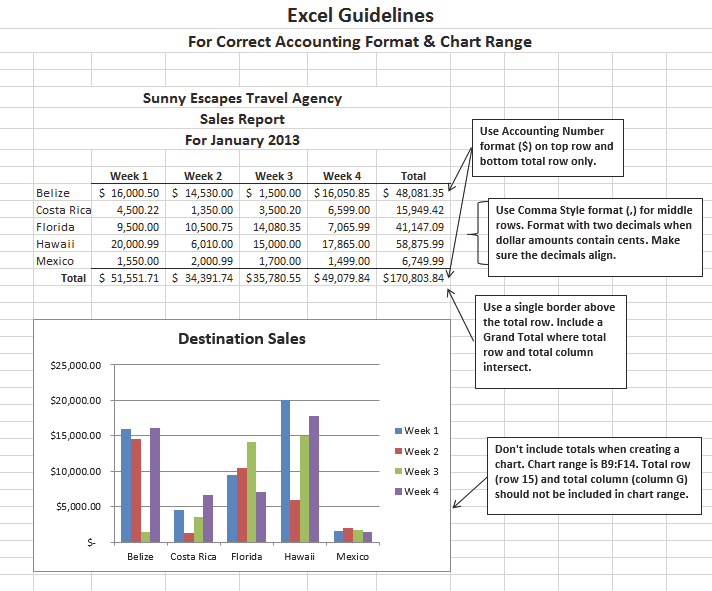
\includegraphics[width=\maxwidth{.95\linewidth}]{gfx/ch01_fig32}
	\caption{Excel Guidelines for Formatting Currency}
	\label{01:fig32}
\end{figure}

Often, Excel spreadsheet contain values that are both currency and non-currency in nature. When that is the case, use the guidelines in Figure \ref{01:fig33}.

\begin{figure}[H]
	\centering
	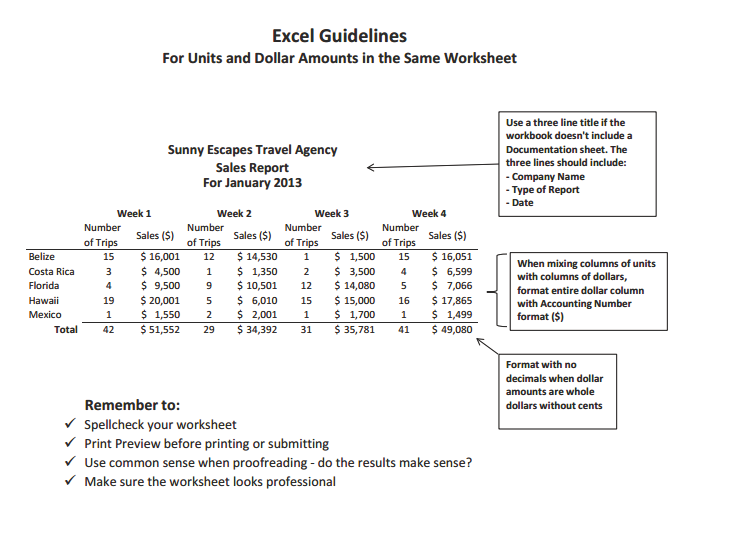
\includegraphics[width=\maxwidth{.95\linewidth}]{gfx/ch01_fig33}
	\caption{Excel Guidelines for Formatting Numbers}
	\label{01:fig33}
\end{figure}

The following steps demonstrate several fundamental formatting skills that will be applied to the workbook developed for this chapter. Several of these formatting skills are identical to ones that may have been used in other Microsoft applications such as Microsoft\textsuperscript{\textregistered} Word\textsuperscript{\textregistered} or Microsoft\textsuperscript{\textregistered} PowerPoint\textsuperscript{\textregistered}.

\begin{enumerate}
	\item Highlight the range \fmtLoc{A2:D2} in the \fmtWorksheet{Sheet1} worksheet by placing the mouse pointer over cell \fmtLoc{A2} and left clicking and dragging to cell \fmtLoc{D2}. 
	\item Click \fmtButton{Home $ \Rightarrow $ Font $ \Rightarrow $ Bold} (see Figure \ref{01:fig34}).
	\item Click \fmtButton{Home $ \Rightarrow $ Font $ \Rightarrow $ Border $ \Rightarrow $ Down Arrow}. Select the \fmtButton{Bottom Border} option from the list to place a border on the bottom of \fmtLoc{Row $ 2 $}.
\end{enumerate}

\begin{figure}[H]
	\centering
	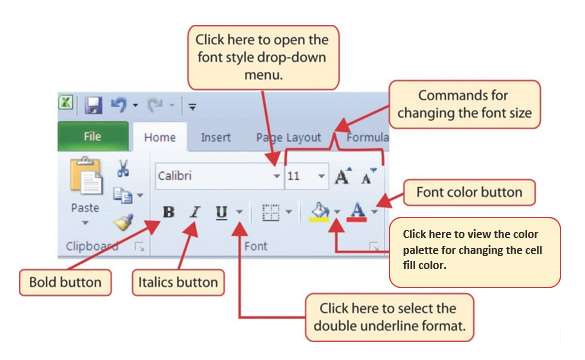
\includegraphics[width=\maxwidth{.95\linewidth}]{gfx/ch01_fig34}
	\caption{Font Group of Commands}
	\label{01:fig34}
\end{figure}

\begin{center}
	\begin{shtcutbox}{Keyboard Shortcuts}
		\textbf{Text Formats}
		\\
		\begin{itemize}
			\setlength{\itemsep}{0pt}
			\setlength{\parskip}{0pt}
			\setlength{\parsep}{0pt}
			
			\item Bold: hold the \fmtKeystroke{Ctrl} key while pressing the letter \fmtKeystroke{B} on the keyboard.
			\item Italics: hold the \fmtKeystroke{Ctrl} key while pressing the letter \fmtKeystroke{I} on the keyboard.
			\item Underline: hold the \fmtKeystroke{Ctrl} key while pressing the letter \fmtKeystroke{U} on the keyboard.
			
		\end{itemize}
	\end{shtcutbox}
\end{center}

\begin{enumerate}[resume]
	\item Highlight the range \fmtLoc{A15:D15} by placing the mouse pointer over cell \fmtLoc{A15} and left clicking and dragging to cell \fmtLoc{D15}.
	\item Click \fmtButton{Home $ \Rightarrow $ Font $ \Rightarrow $ Bold}.
	\item Click \fmtButton{Home $ \Rightarrow $ Font $ \Rightarrow $ Border $ \Rightarrow $ Down Arrow}. Select the \fmtButton{Top Border} option from the list to place a border on the top of \fmtLoc{Row $ 15 $} where totals will eventually be displayed.
	\item Highlight the range \fmtLoc{B3:B14} by placing the mouse pointer over cell \fmtLoc{B3} and left clicking and dragging down to cell \fmtLoc{B14}.
	\item Click \fmtButton{Home $ \Rightarrow $ Number $ \Rightarrow $ Comma Style}. This feature adds a comma and two decimal places to numbers in the cell. (see Figure \ref{01:fig35}).
\end{enumerate}

\begin{figure}[H]
	\centering
	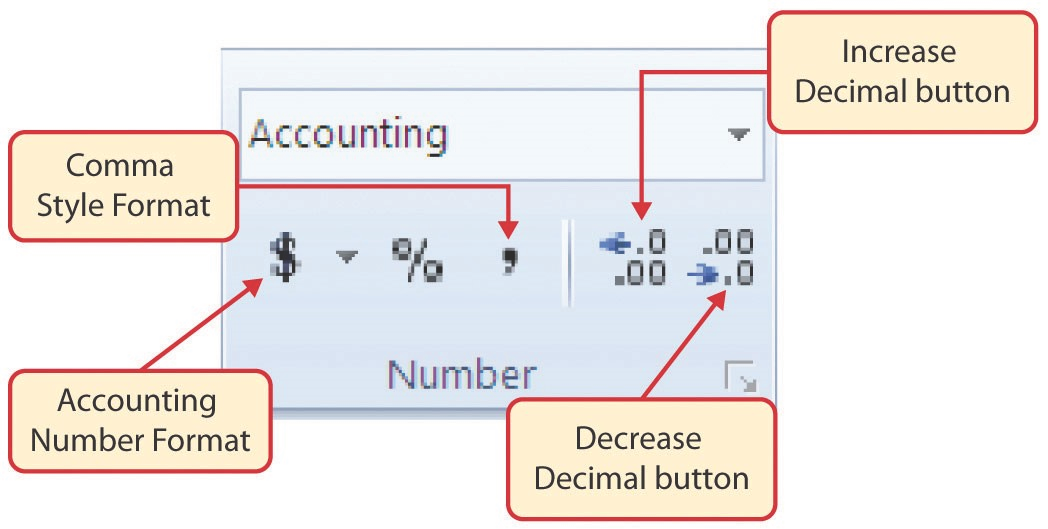
\includegraphics[width=\maxwidth{.95\linewidth}]{gfx/ch01_fig35}
	\caption{Number Group of Commands}
	\label{01:fig35}
\end{figure}

\begin{center}
	\begin{infobox}{Why?}
		\textbf{Format Column Headings and Totals}
		\\
		\\
		Applying formatting enhancements to the column headings and column totals in a worksheet is a very important technique, especially if the workbook will be shared with other people. These formatting techniques allow users of the worksheet to clearly see the column headings that define the data. In addition, the column totals usually contain the most important data on a worksheet with respect to making decisions, and formatting techniques allow users to quickly find this information.
	\end{infobox}
\end{center}


\begin{enumerate}[resume]
	\item Since the figures in this range do not include cents, click \fmtButton{Home $ \Rightarrow $ Number $ \Rightarrow $ Decrease Decimal} two times (see Figure \ref{01:fig35}).
	\item The numbers will be reduced to zero decimal places.
	\item Highlight the range \fmtLoc{C3:C14} by placing the mouse pointer over cell \fmtLoc{C3} and left clicking and dragging down to cell \fmtLoc{C14}.
	\item Click \fmtButton{Home $ \Rightarrow $ Number $ \Rightarrow $ Accounting Number} (see Figure \ref{01:fig35}). This will add a currency symbol and two decimal places to the values, which is common when working with pricing data. As discussed in the Formatting Data and Cells section above, use Accounting format on all values in this range since the worksheet contains non-currency as well as currency data.
	\item Highlight the range \fmtLoc{D3:D14} by placing the mouse pointer over cell \fmtLoc{D3} and left clicking and dragging down to cell \fmtLoc{D14}.
	\item Apply the Accounting Number Format to add the US currency symbol to the values and set them for two decimal places.
	\item Click \fmtButton{Home $ \Rightarrow $ Number $ \Rightarrow $ Decrease Decimal} two times to reduce the decimal places to zero since there are no cents in these figures.
	\item Highlight the range \fmtLoc{A1:D1} by placing the mouse pointer over cell \fmtLoc{A1} and left clicking and dragging over to cell \fmtLoc{D1}.
	\item Click \fmtButton{Home $ \Rightarrow $ Font $ \Rightarrow $ Fill Color $ \Rightarrow $ Down Arrow} (see Figure \ref{01:fig36}). This will prepare the range for a worksheet title.
\end{enumerate}

\begin{figure}[H]
	\centering
	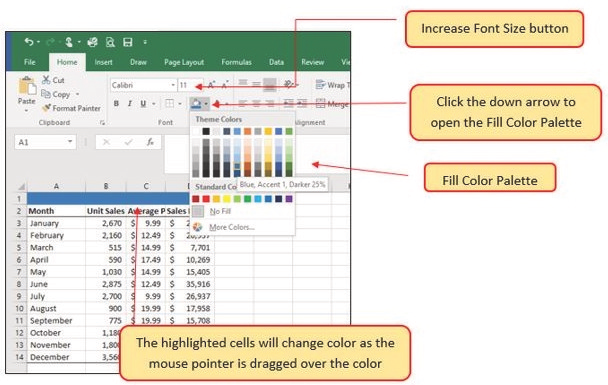
\includegraphics[width=\maxwidth{.95\linewidth}]{gfx/ch01_fig36}
	\caption{Fill Color Palette}
	\label{01:fig36}
\end{figure}

\begin{enumerate}[resume]
	\item Click the \textit{Blue, Accent 1, Darker 25\%} color from the palette (see Figure \ref{01:fig36}). Notice that as the mouse pointer moves over the color palette, a preview of the color appears in the highlighted cells. That makes it easy to experiment with various colors.
	\item Click on \fmtLoc{A1} and enter the worksheet title, \fmtTyping{General Merchandise World}.
	\item Click on \fmtLoc{A2} and then click on \fmtLoc{A1}.This is necessary to select the cell that contains the text rather than the text itself.
	\item Since the black font is difficult to read on the blue background, change the font color to be more visible. Click \fmtButton{Home $ \Rightarrow $ Font $ \Rightarrow $ Font Color $ \Rightarrow $ Down Arrow} and select \textit{White} as the font color for this range (see Figure \ref{01:fig34}).
	\item Highlight the range \fmtLoc{A1:D15} by placing the mouse pointer over cell \fmtLoc{A1} and left clicking and dragging down to cell \fmtLoc{D15}.
	\item Click \fmtButton{Home $ \Rightarrow $ Font $ \Rightarrow $ Down Arrow} and select \textit{Arial} as the font for this range. (see Figure \ref{01:fig34}). Notice that as the mouse pointer moves over the font style options, it changes the highlighted cells. This makes it easy to preview various font options before they are applied.
	\item Expand the column width of \fmtLoc{Column D} to $ 14 $ characters.
\end{enumerate}

Figure \ref{01:fig37} shows how the \fmtWorksheet{Sheet1} worksheet should appear after the formatting techniques are applied.

\begin{figure}[H]
	\centering
	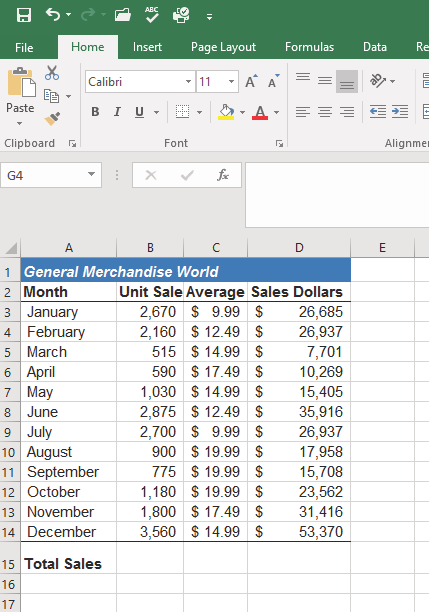
\includegraphics[width=\maxwidth{.95\linewidth}]{gfx/ch01_fig37}
	\caption{Formatting Techniques Applied}
	\label{01:fig37}
\end{figure}

\begin{center}
	\begin{infobox}{Why}
		\textbf{Hashtags (\#\#\#\#) Appear in Columns}
		\\
		\\
		When a column is too narrow for a long number, Excel will automatically convert the number to a series of hashtags (\#\#\#\#). In the case of words or text data, Excel will only show the characters that fit in the column. However, this is not the case with numeric data because it can give the appearance of a number that is much smaller than what is actually in the cell. To remove the hashtags, increase the width of the column.
	\end{infobox}
\end{center}


\subsection{Data Alignment (Wrap Text, Merge Cells, and Center)}

The skills presented in this section show how data is aligned within cell locations. For example, text and numbers can be centered, left aligned, right aligned, and so on within a cell. In some cases multi-word text entries may need to be stacked vertically instead of expanding the width of a column, which is referred to as wrapping text. These skills are demonstrated in the following steps.

\begin{enumerate}
	\item Highlight the range \fmtLoc{B2:D2} by placing the mouse pointer over cell \fmtLoc{B2} and left clicking and dragging over to cell \fmtLoc{D2}.
	\item Click \fmtButton{Home $ \Rightarrow $ Alignment $ \Rightarrow $ Center} (see Figure \ref{01:fig38}). This will center the column headings in each cell location. Notice the difference between text that is centered horizontally and text that is middle aligned vertically.
\end{enumerate}

\begin{figure}[H]
	\centering
	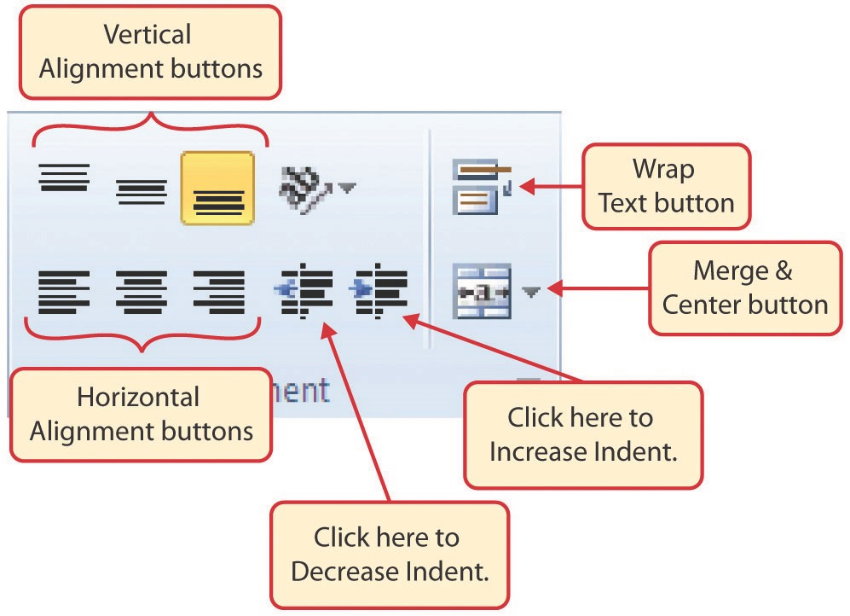
\includegraphics[width=\maxwidth{.95\linewidth}]{gfx/ch01_fig38}
	\caption{Alignment Group in Home Tab}
	\label{01:fig38}
\end{figure}

\begin{enumerate}[resume]
	\item Click \fmtButton{Home $ \Rightarrow $ Alignment $ \Rightarrow $ Wrap Text} (see Figure \ref{01:fig38}). The height of \fmtLoc{Row $ 2 $} automatically expands, and the words that were cut off because the columns were too narrow are now stacked vertically.
\end{enumerate}

\begin{center}
	\begin{shtcutbox}{Keyboard Shortcuts}
		\textbf{Wrap Text}
		\\
		\begin{itemize}
			\setlength{\itemsep}{0pt}
			\setlength{\parskip}{0pt}
			\setlength{\parsep}{0pt}
			
			\item Press the \fmtKeystroke{Alt} key and then the letters \fmtKeystroke{H} and \fmtKeystroke{W} one at a time.
			
		\end{itemize}
	\end{shtcutbox}
\end{center}

\begin{enumerate}[resume]
	\item Highlight the range \fmtLoc{A1:D1} by placing the mouse pointer over cell \fmtLoc{A1} and left clicking and dragging over to cell \fmtLoc{D1}.
	\item Click \fmtButton{Home $ \Rightarrow $ Alignment $ \Rightarrow $ Merge \& Center $ \Rightarrow $ Down Arrow}.
	\item Click the \fmtButton{Merge \& Center} option (see Figure \ref{01:fig39}). This will create one large cell location running across the top of the data set.

\end{enumerate}

\begin{figure}[H]
	\centering
	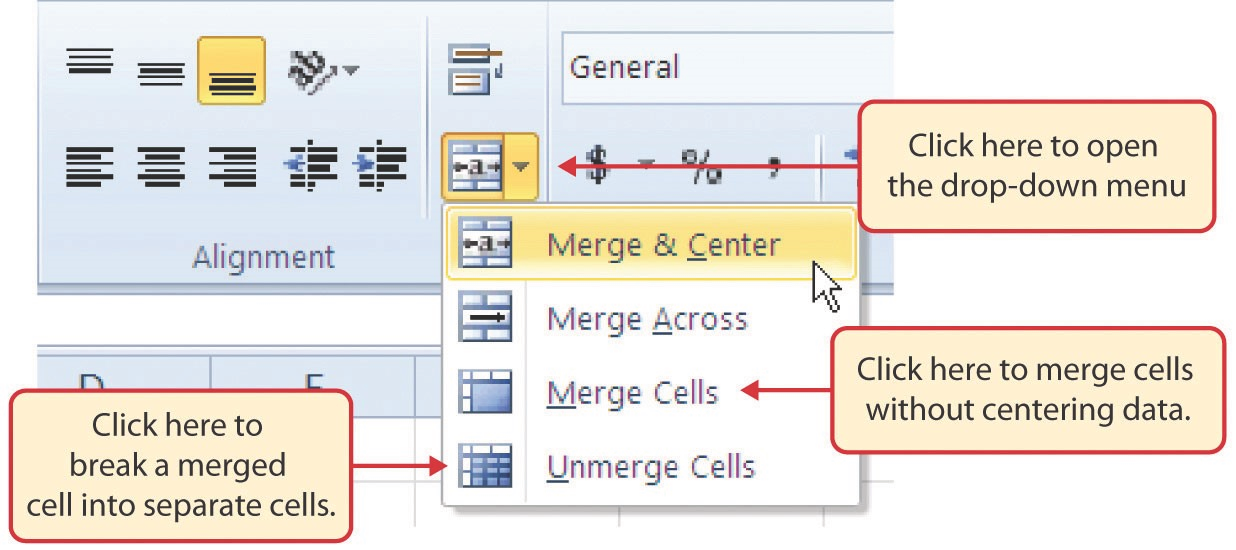
\includegraphics[width=\maxwidth{.95\linewidth}]{gfx/ch01_fig39}
	\caption{Merge Cell Drop-Down Menu}
	\label{01:fig39}
\end{figure}

\begin{center}
	\begin{shtcutbox}{Keyboard Shortcuts}
		\textbf{Merge Commands}
		\\
		\begin{itemize}
			\setlength{\itemsep}{0pt}
			\setlength{\parskip}{0pt}
			\setlength{\parsep}{0pt}
			
			\item \textbf{Merge \& Center}: Press the \fmtKeystroke{Alt} key and then the letters \fmtKeystroke{H}, \fmtKeystroke{M}, and \fmtKeystroke{C} one at a time.
			\item \textbf{Merge Cells}: Press the \fmtKeystroke{Alt} key and then the letters \fmtKeystroke{H}, \fmtKeystroke{M}, and \fmtKeystroke{M} one at a time.
			\item \textbf{Unmerge Cells}: Press the \fmtKeystroke{Alt} key and then the letters \fmtKeystroke{H}, \fmtKeystroke{M}, and \fmtKeystroke{U} one at a time.
			
		\end{itemize}
	\end{shtcutbox}
\end{center}

\begin{center}
	\begin{infobox}{Why?}
		\textbf{Wrap Text}
		\\
		\\
		The benefit of using the Wrap Text command is that it significantly reduces the need to expand the column width to accommodate multi-word column headings. The problem with increasing the column width is that it may reduce the amount of data that can fit on a piece of paper or one screen. This makes it cumbersome to analyze the data in the worksheet and could increase the time it takes to make a decision.
	\end{infobox}
\end{center}

Figure \ref{01:fig40} shows the \textit{Sheet1} worksheet with the data alignment commands applied. The reason for merging the cells in the range $ A1 $:$ D1 $ will become apparent in the next section.

\begin{figure}[H]
	\centering
	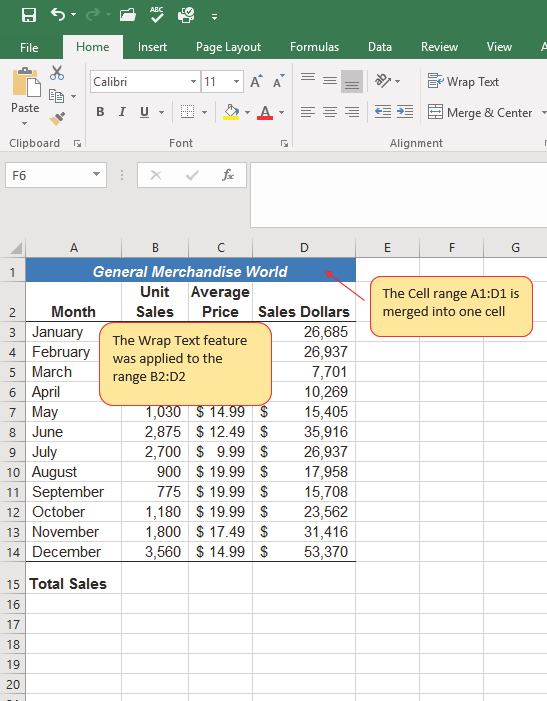
\includegraphics[width=\maxwidth{.95\linewidth}]{gfx/ch01_fig40}
	\caption{Sheet1 with Data Alignment Features Added}
	\label{01:fig40}
\end{figure}

\begin{center}
	\begin{infobox}{Why?}
		\textbf{Merge \& Center}
		\\
		\\
		One of the most common reasons the \fmtButton{Merge \& Center} command is used is to center the title of a worksheet directly above the columns of data. Once the cells above the column headings are merged, a title can be centered above the columns of data. It is very difficult to center the title over the columns of data if the cells are not merged.
	\end{infobox}
\end{center}

\begin{center}
	\begin{sklbox}{Skill Refresher}
		\textbf{Wrap Text}
		\\
		\begin{itemize}
			\setlength{\itemsep}{0pt}
			\setlength{\parskip}{0pt}
			\setlength{\parsep}{0pt}
			
			\item Activate the cell or range of cells that contain text data.
			\item Click \fmtButton{Home $ \Rightarrow $ Alignment $ \Rightarrow $ Wrap Text}.

		\end{itemize}
	\end{sklbox}
\end{center}

\begin{center}
	\begin{sklbox}{Skill Refresher}
		\textbf{Merge Cells}
		\\
		\begin{itemize}
			\setlength{\itemsep}{0pt}
			\setlength{\parskip}{0pt}
			\setlength{\parsep}{0pt}
			
			\item Highlight a range of cells that will be merged.
			\item Click \fmtButton{Home $ \Rightarrow $ Alignment $ \Rightarrow $ Merge \& Center Down Arrow}.
			\item Select an option from the \fmtButton{Merge \& Center} list.
			
		\end{itemize}
	\end{sklbox}
\end{center}

\subsection{Entering Multiple Lines of Text}

In the \textit{Sheet1} worksheet, the cells in the range $ A1 $:$ D1 $ were merged for the purposes of adding a title to the worksheet. This worksheet will contain both a title and a subtitle. The following steps explain how to enter text into a cell and determine where the second line of text should begin.

\begin{enumerate}
	\item Click cell \fmtLoc{A1} in the \fmtWorksheet{Sheet1} worksheet. Since the cells were merged, clicking cell \fmtLoc{A1} will automatically activate the range \fmtLoc{A1:D1}. Position the mouse to the end of the title, directly after the ``d'' in the word ``World'' and double-click to get a cursor (flashing I-beam).
	\item Hold down the \fmtKeystroke{Alt} key and press the \fmtKeystroke{Enter} key. This will start a new line of text in this cell location.
	\item Type the text \fmtTyping{Retail Sales (in millions)} and press the \fmtKeystroke{Enter} key.
	\item Click cell \fmtLoc{A1}. 
	\item Increase the height of Row $ 1 $ to $ 30 $ points. Once the row height is increased, all the text typed into the cell will be visible (see Figure \ref{01:fig41}).
	\item Click \fmtButton{Home $ \Rightarrow $ Font $ \Rightarrow $ Bold}.
	\item Click \fmtButton{Home $ \Rightarrow $ Font $ \Rightarrow $ Italics}.

\end{enumerate}

\begin{figure}[H]
	\centering
	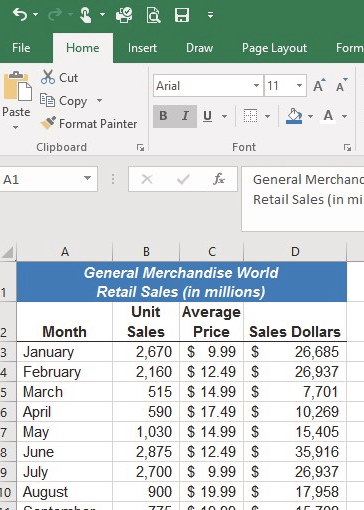
\includegraphics[width=\maxwidth{.95\linewidth}]{gfx/ch01_fig41}
	\caption{Title \& Subtitle Added to the Worksheet}
	\label{01:fig41}
\end{figure}

\begin{center}
	\begin{sklbox}{Skill Refresher}
		\textbf{Entering Multiple Lines of Text}
		\\
		\begin{itemize}
			\setlength{\itemsep}{0pt}
			\setlength{\parskip}{0pt}
			\setlength{\parsep}{0pt}
			
			\item Activate a cell location.
			\item Type the first line of text.
			\item Hold down the \fmtKeystroke{Alt} key and press the \fmtKeystroke{Enter} key.
			\item Type the second line of text and press the \fmtKeystroke{Enter} key.
			
		\end{itemize}
	\end{sklbox}
\end{center}

\subsection{Borders (Adding Lines to a Worksheet)}

In Excel, adding custom lines to a worksheet is known as adding borders. Borders are different from the grid lines that appear on a worksheet and that define the perimeter of the cell locations. Borders add a variety of line styles to a worksheet that can make reading the worksheet much easier. The following steps illustrate methods for adding both preset and custom borders to a worksheet.

\begin{enumerate}
	\item Click \fmtButton{Home $ \Rightarrow $ Font $ \Rightarrow $ Borders $ \Rightarrow $ Down Arrow} to view border options. (see Figure \ref{01:fig42}).
\end{enumerate}

\begin{figure}[H]
	\centering
	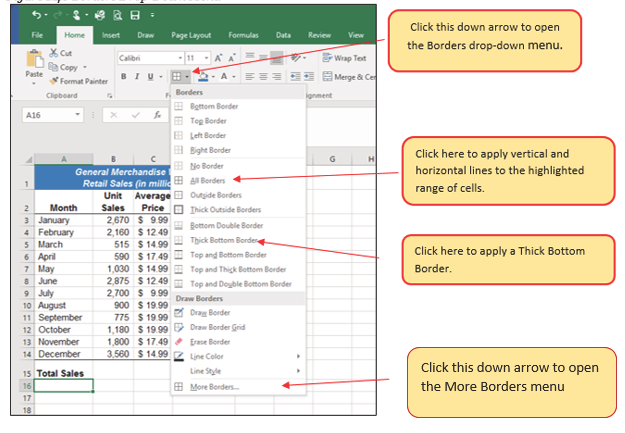
\includegraphics[width=\maxwidth{.95\linewidth}]{gfx/ch01_fig42}
	\caption{Borders Drop-Down Menu}
	\label{01:fig42}
\end{figure}

\begin{enumerate}[resume]
	\item Highlight the range \fmtLoc{A1:D15}. 
	\item Click \fmtButton{Home $ \Rightarrow $ Font $ \Rightarrow $ Borders $ \Rightarrow $ Down Arrow $ \Rightarrow $ All Borders} (see Figure \ref{01:fig42}). This will add vertical and horizontal lines to the range \fmtLoc{A1:D15}.
	\item Highlight the range \fmtLoc{A2:D2} by clicking \fmtLoc{A2} and dragging to cell \fmtLoc{D2}.
	\item Click \fmtButton{Home $ \Rightarrow $ Font $ \Rightarrow $ Borders $ \Rightarrow $ Down Arrow $ \Rightarrow $ Thick Bottom Border}
	\item Highlight the range \fmtLoc{A14:D14} and click \fmtButton{Home $ \Rightarrow $ Font $ \Rightarrow $ Borders $ \Rightarrow $ Down Arrow $ \Rightarrow $ Thick Bottom Border}. The thick border will help maintain the \textit{Excel Formatting Guidelines}.
	\item Highlight the range \fmtLoc{A1:D15}.
	\item Click \fmtButton{Home $ \Rightarrow $ Font $ \Rightarrow $ Borders $ \Rightarrow $ Down Arrow $ \Rightarrow $ More Borders...}
	\item This will open the \textit{Format Cells} dialog box (see Figure \ref{01:fig43}). All Excel formatting commands can be accessed through this dialog box.
	\item In the \textit{Style} section of the \textit{Borders} tab, click the thickest line style (see Figure \ref{01:fig43}).
	\item Click the \fmtButton{Outline} button in the \textit{Presets} section (see Figure \ref{01:fig43}).
	\item Click the \fmtButton{OK} button at the bottom of the dialog box (see Figure \ref{01:fig43}).
\end{enumerate}

\begin{figure}[H]
	\centering
	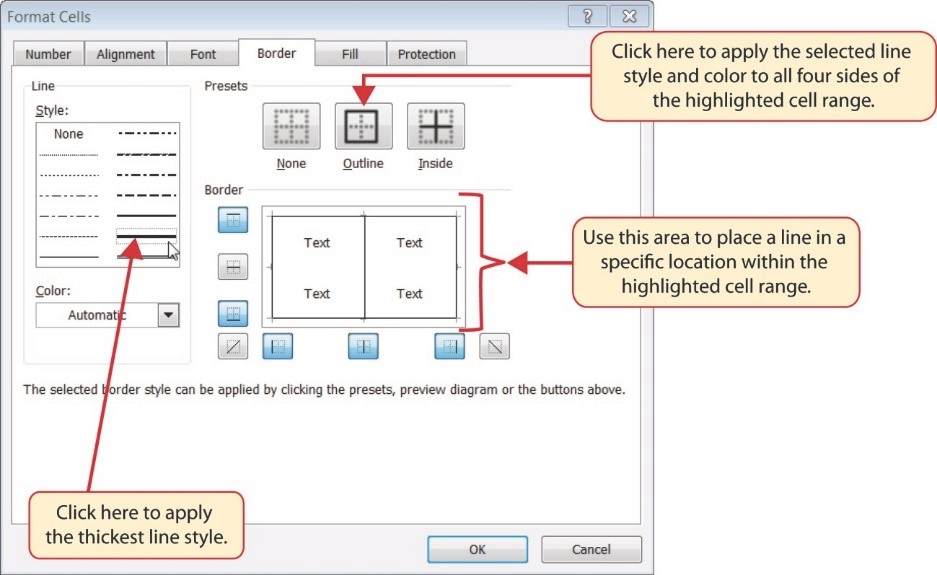
\includegraphics[width=\maxwidth{.95\linewidth}]{gfx/ch01_fig43}
	\caption{Borders Tab of the Format Cells Dialog Box}
	\label{01:fig43}
\end{figure}

The \textit{Sheet1} worksheet should now look like Figure \ref{01:fig44}.

\begin{figure}[H]
	\centering
	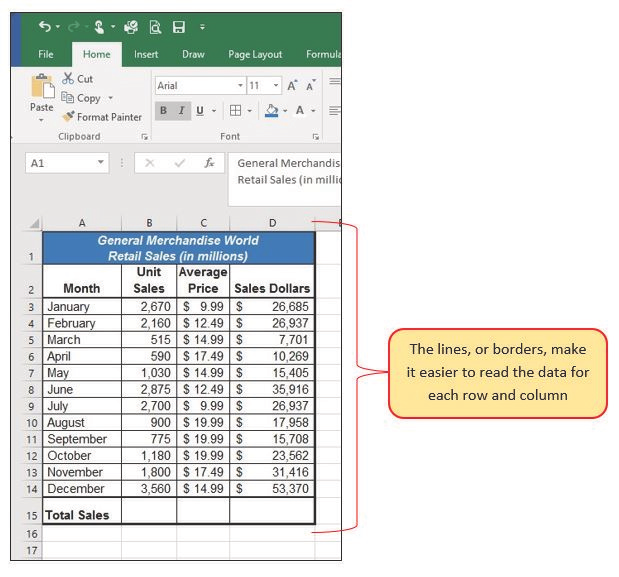
\includegraphics[width=\maxwidth{.95\linewidth}]{gfx/ch01_fig44}
	\caption{Borders Added to the Sheet1 Worksheet}
	\label{01:fig44}
\end{figure}

\begin{center}
	\begin{sklbox}{Skill Refresher}
		\textbf{Preset Borders}
		\\
		\begin{itemize}
			\setlength{\itemsep}{0pt}
			\setlength{\parskip}{0pt}
			\setlength{\parsep}{0pt}
			
			\item Highlight a range of cells that require borders.
			\item Click the \fmtButton{Home} tab of the Ribbon.
			\item Click the down arrow next to the \fmtButton{Borders} button.
			\item Select an option from the preset borders list.
			
		\end{itemize}

		\hfill \break
		\textbf{Custom Borders}
		\\
		\begin{itemize}
			\setlength{\itemsep}{0pt}
			\setlength{\parskip}{0pt}
			\setlength{\parsep}{0pt}
			
			\item Highlight a range of cells that require borders.
			\item Click \fmtButton{Home $ \Rightarrow $ Font $ \Rightarrow $ Borders $ \Rightarrow $ Down Arrow $ \Rightarrow $ More Borders...}
			\item Select a line style and line color.
			\item Select a placement option.
			\item Click the \fmtButton{OK} button on the dialog box.
			
		\end{itemize}

	\end{sklbox}
\end{center}

\subsection{Autosum}

Notice at the bottom of Figure \ref{01:fig44} that \textit{Row 15} is intended to show the totals for the data in this worksheet. Applying mathematical computations to a range of cells is accomplished through functions in Excel. Chapter \ref{ch03:formulas}, \nameref{ch03:formulas}, page \pageref{ch03:formulas}, in this book reviews mathematical formulas and functions in detail; however, the following steps will demonstrate how to quickly sum the values in a column of data using the AutoSum command.

\begin{enumerate}
	\item Click in cell \fmtLoc{B15} in the \fmtWorksheet{Sheet1} worksheet.
	\item Click \fmtButton{Formulas $ \Rightarrow $ Function Library $ \Rightarrow $ AutoSum $ \Rightarrow $ Down Arrow} (see Figure \ref{01:fig45}). Note that autosum can also be found at \fmtButton{Home $ \Rightarrow $ Editing $ \Rightarrow $ AutoSum}.
\end{enumerate}

\begin{figure}[H]
	\centering
	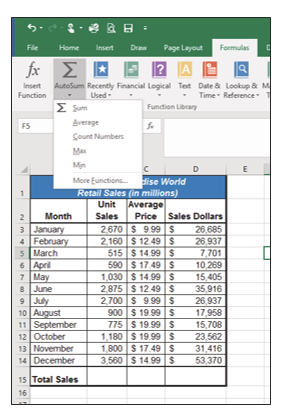
\includegraphics[width=\maxwidth{.95\linewidth}]{gfx/ch01_fig45}
	\caption{AutoSum Drop-Down List}
	\label{01:fig45}
\end{figure}

\begin{enumerate}[resume]
	\item Click the \fmtButton{Sum} option from the \textit{AutoSum} drop-down menu. The first click will display a flashing marquee around the range. Press the \fmtKeystroke{Enter} key or click the \fmtButton{Check Mark} next to the Formula bar to complete the function.
	\item Excel will provide a total for the values in the \textit{Unit Sales} column.
	\item It would not make sense to total the averages in \fmtLoc{Column C} so \fmtLoc{C15} will be left blank.
	\item Click in cell \fmtLoc{D15}. 
	\item Click \fmtButton{Formulas $ \Rightarrow $ Function Library $ \Rightarrow $ AutoSum $ \Rightarrow $ Down Arrow}. 
	\item Click the \fmtButton{Sum} option from the \textit{AutoSum} drop-down menu. The first click will display a flashing marquee around the range. Press the \fmtKeystroke{Enter} key or click the \fmtButton{Check Mark} next to the Formula bar to complete the function. (see Figure \ref{01:fig46}).
\end{enumerate}

\begin{figure}[H]
	\centering
	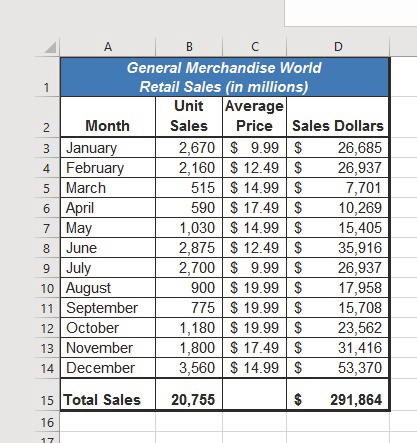
\includegraphics[width=\maxwidth{.95\linewidth}]{gfx/ch01_fig46}
	\caption{Totals Added to the Sheet1 Worksheet}
	\label{01:fig46}
\end{figure}

\begin{center}
	\begin{sklbox}{Skill Refresher}
		\textbf{AutoSum}
		\\
		\begin{itemize}
			\setlength{\itemsep}{0pt}
			\setlength{\parskip}{0pt}
			\setlength{\parsep}{0pt}
			
			\item Highlight a cell location below or to the right of a range of cells that contain numeric values.
			\item Click the \fmtButton{Formulas} tab of the Ribbon.
			\item Click the down arrow below the \fmtButton{AutoSum} button.
			\item Select a mathematical function from the list.
			
		\end{itemize}
	\end{sklbox}
\end{center}

\subsection{Moving, Renaming, Inserting, and Deleting Worksheets}

The default names for the worksheet tabs at the bottom of workbook are \textit{Sheet1}, \textit{Sheet2}, and so on. However, the worksheet names can be changed to identify the data each worksheet contains. Additionally, the order that the worksheet tabs appear can be changed. The following steps explain how to rename and move the worksheets in a workbook.

\begin{enumerate}
	\item Double-click the \fmtWorksheet{Sheet1} worksheet tab at the bottom of the workbook (see Figure \ref{01:fig47}). 
	\item Type the name \fmtTyping{Sales by Month} and press \fmtKeystroke{Enter}.
	\item Double click the \fmtWorksheet{Sheet2} worksheet tab at the bottom of the workbook.
	\item Type the name \fmtTyping{Unit Sales Rank} and press \fmtKeystroke{Enter}.
\end{enumerate}

\begin{figure}[H]
	\centering
	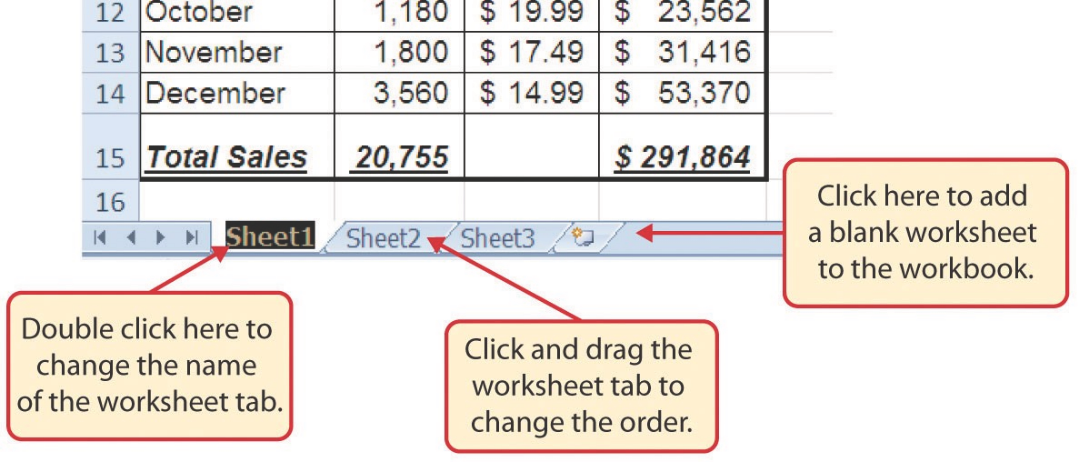
\includegraphics[width=\maxwidth{.95\linewidth}]{gfx/ch01_fig47}
	\caption{Renaming a Worksheet Tab}
	\label{01:fig47}
\end{figure}

\begin{enumerate}
	\item Click-and-drag the \fmtWorksheet{Unit Sales Rank} worksheet tab to the left of the \fmtWorksheet{Sales by Month} sheet. It will become the first worksheet in the workbook.
	\item Click the \fmtWorksheet{Sheet3} worksheet tab.
	\item Click \fmtButton{Home $ \Rightarrow $ Cells $ \Rightarrow $ Delete $ \Rightarrow $ Down Arrow $ \Rightarrow $ Delete Sheet}. This removes the unneeded worksheet.
	\item If a warning box pops up, click the \fmtButton{Delete} button.
	\item Also delete the \fmtWorksheet{Unit Sales Rank} worksheet since it was decided that worksheet is also unnecessary. This means that the workbook is left with just one worksheet, \fmtWorksheet{Sales by Month}.
	\item Save the changes to the workbook by clicking either \fmtButton{Quick Access Toolbar $ \Rightarrow $ Save} or \fmtButton{File $ \Rightarrow $ Save}.
\end{enumerate}

\begin{center}
	\begin{infobox}{Integrity Check}
		\textbf{Deleting Worksheets}
		\\
		\\
		Be very cautious when deleting worksheets that contain data. Once a worksheet is deleted it is gone forever; the Undo command cannot bring the sheet back. \textit{Deleting a worksheet is permanent!}
	\end{infobox}
\end{center}

\begin{center}
	\begin{shtcutbox}{Keyboard Shortcuts}
		\textbf{Inserting New Worksheets}
		\\
		\begin{itemize}
			\setlength{\itemsep}{0pt}
			\setlength{\parskip}{0pt}
			\setlength{\parsep}{0pt}
			
			\item Press the \fmtKeystroke{Shift} key and then the \fmtKeystroke{F11} key on the keyboard.
			
		\end{itemize}
	\end{shtcutbox}
\end{center}


Figure \ref{01:fig48} shows the final appearance of the \textit{CH1-GMW Sales} workbook.

\begin{figure}[H]
	\centering
	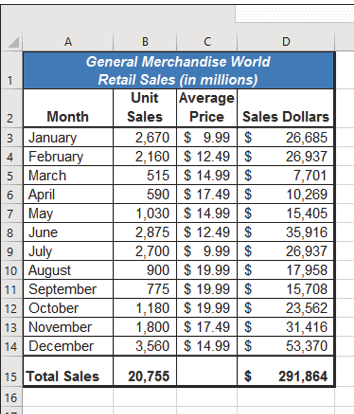
\includegraphics[width=\maxwidth{.95\linewidth}]{gfx/ch01_fig48}
	\caption{Final Appearance of the CH1-GMW Sales Workbook}
	\label{01:fig48}
\end{figure}

\begin{center}
	\begin{sklbox}{Skill Refresher}
		\textbf{Renaming Worksheets}
		\\
		\begin{itemize}
			\setlength{\itemsep}{0pt}
			\setlength{\parskip}{0pt}
			\setlength{\parsep}{0pt}
			
			\item Double click the worksheet tab.
			\item Type the new name.
			\item Press the \fmtKeystroke{Enter} key.
		\end{itemize}

		\hfill \break
		\textbf{Moving Worksheets}
		\\
		\begin{itemize}
			\setlength{\itemsep}{0pt}
			\setlength{\parskip}{0pt}
			\setlength{\parsep}{0pt}
			
			\item Left click the worksheet tab.
			\item Drag it to the desired position.
		\end{itemize}

		\hfill \break
		\textbf{Deleting Worksheets}
		\\
		\begin{itemize}
			\setlength{\itemsep}{0pt}
			\setlength{\parskip}{0pt}
			\setlength{\parsep}{0pt}
			
			\item Open the worksheet to be deleted.
			\item Click \fmtButton{Home $ \Rightarrow $ Cells $ \Rightarrow $ Delete $ \Rightarrow $ Down Arrow $ \Rightarrow $ Delete Sheet}.
			\item Click \fmtButton{Delete} on the warning box.
		\end{itemize}

	\end{sklbox}
\end{center}

\begin{center}
	\begin{infobox}{Best Practice}
		\textbf{Summary Worksheet}
		\\
		\\
		It is considered a best practice to make the first worksheet in a workbook a summary. That sheet should include the purpose of the workbook and a brief explanation for each of the sheets in the book. It should also include contact information for the originator so questions that may come up later can be clarified. The simple workbooks in this course will not include a summary sheet, but it would be included in more complex projects.
	\end{infobox}
\end{center}


\begin{center}
	\begin{tkwbox}{Key Take-Aways}
		\textbf{Save}
		\\
		\begin{itemize}
			\setlength{\itemsep}{0pt}
			\setlength{\parskip}{0pt}
			\setlength{\parsep}{0pt}
			
			\item Formatting skills are critical for creating worksheets that are easy to read and have a professional appearance.
			\item A series of hashtags (\#\#\#\#) in a cell location indicates that the column is too narrow to display the number entered.
			\item Using the Wrap Text command allows multi-word column headings to be stacked vertically in a cell location, reducing the need to expand column widths.
			\item Use the \textit{Merge \& Center} command to center the title of a worksheet directly over the columns that contain data.
			\item Adding borders or lines will make the worksheet easier to read and helps to separate the data in each column and row.
			\item The Undo command will not bring back a worksheet that has been deleted.
		
		\end{itemize}
	\end{tkwbox}
\end{center}

\section{Printing}

\begin{center}
	\begin{objbox}{Learning Objectives}
		\begin{itemize}
			\setlength{\itemsep}{0pt}
			\setlength{\parskip}{0pt}
			\setlength{\parsep}{0pt}
			
			\item Use the \textit{Page Layout} tab to prepare a worksheet for printing.
			\item Add headers and footers to a printed worksheet.
			\item Explore how to print worksheets and workbooks.
		\end{itemize}
	\end{objbox}
\end{center}

Once a workbook is completed, it is good practice to select the appropriate settings for printing. These settings are in the \textit{Page Layout} tab of the Ribbon and discussed in this section of the chapter.

\subsection{Page Setup}

Before the worksheets in a workbook can be properly printed, the setting must be adjusted. The following steps explain several of the commands in the \textit{Page Layout} tab of the Ribbon used to prepare a worksheet for printing.

\begin{enumerate}
	\item Open the \fmtWorksheet{CH1-GMW Sales} workbook if it is not already open.
	\item Click \fmtButton{Page Layout $ \Rightarrow $ Page Setup $ \Rightarrow $ Margins}. This will open a drop-down list of options for setting the margins of the printed document. The \fmtButton{Normal}, \fmtButton{Wide}, and \fmtButton{Narrow} will quickly apply one of those common margin settings and for this worksheet, click \fmtButton{Narrow}.
	\item To further adjust the margin settings, \fmtButton{Page Layout $ \Rightarrow $ Page Setup $ \Rightarrow $ Margins $ \Rightarrow $ Custom Margins}.
	\item On the \textit{Page Setup} dialog box, click the \fmtButton{Page} tab, then select \fmtButton{Landscape}.
	\item Click the \textit{Margins} tab and locate the \fmtButton{Center on Page} section. Click the boxes to Horizontally and Vertically center the data on the worksheet. (see Figure \ref{01:fig49})
	\item Click \fmtButton{OK}.
\end{enumerate}

\begin{figure}[H]
	\centering
	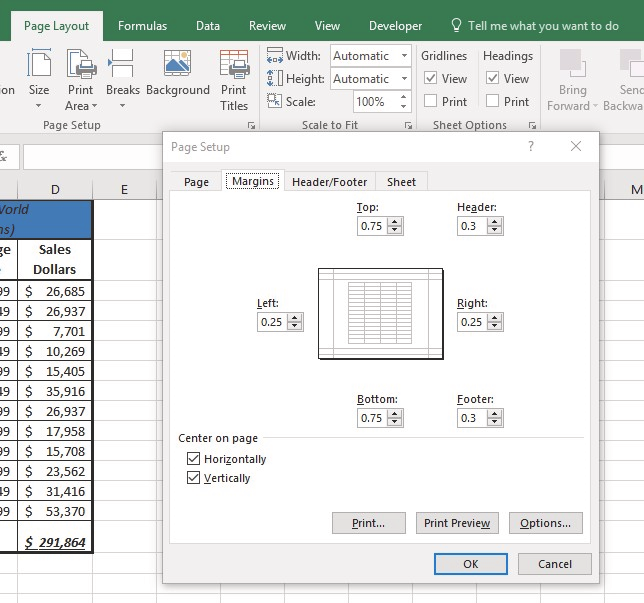
\includegraphics[width=\maxwidth{.95\linewidth}]{gfx/ch01_fig49}
	\caption{Page Layout Commands for Printing}
	\label{01:fig49}
\end{figure}

\begin{center}
	\begin{infobox}{Why?}
		\textbf{Use Print Settings}
		\\
		\\
		Because professionals often share Excel workbooks, it is a good practice to select the appropriate print settings in the \textit{Page Layout} tab even if there is no intent to print the worksheets. It can be extremely frustrating for recipients of a workbook who wish to print the worksheets to find that the necessary print settings have not been selected. 
	\end{infobox}
\end{center}

Table \ref{01:tab02} lists the various page layout settings and how they would be used.

\begin{table}[H]
	\rowcolors{1}{}{tablerow} % zebra striping background
	{\fontsize{8}{10} \selectfont %\small
		%\fontsize{8}{10} \selectfont %Replace small for special font size
		\begin{longtable}{L{0.75in}L{1.75in}L{1.75in}} %Left-aligned, Max width: 4.25in
			\textbf{Command} & \textbf{Purpose} & \textbf{Use} \endhead
			\hline
			Margins & Sets the top, bottom, right, and left margin space for the printed document & 1. Click the Page Layout tab of the Ribbon.\newline2. Click the Margin button.\newline3. Click one of the preset margin options or click Custom Margins.\\
			Orientation & Sets the orientation of the printed document to either portrait or landscape & 1. Click the Page Layout tab of the Ribbon.\newline2. Click the Orientation button.\newline3. Click one of the preset orientation options.\\
			Size & Sets the paper size for the printed document & 1. Click the Page Layout tab of the Ribbon.\newline2. Click the Size button.\newline3. Click one of the preset paper size options or click More Paper Sizes. \\
			Print Area & Used for printing only a specific area or range of cells on a worksheet & 1. Highlight the range of cells on a worksheet to be printed.\newline2. Click the Page Layout tab of the Ribbon.\newline3. Click the Print Area button.\newline4. Click the Set Print Area option from the drop-down list. \\
			Breaks & Manually set the page breaks on a worksheet & 1. Activate a cell on the worksheet where the page break should be placed. Breaks are created above and to the left of the activated cell.\newline2. Click the Page Layout tab of the Ribbon.\newline3. Click the Breaks button.\newline4. Click the Insert Page Break option from the drop-down list. \\
			Background & Adds a picture behind the cell locations in a worksheet & 1. Click the Page Layout tab of the Ribbon.\newline2. Click the Background button.\newline3. Select a picture stored on the local computer or network. \\
			Print Titles & Used when printing large data sets that are several pages long. This command will repeat the column headings at the top of each printed page. & 1. Click the Page Layout tab of the Ribbon.\newline2. Click the Print Titles button.\newline3. Click in the Rows to Repeat at Top input box in the Page Setup dialog box.\newline4. Click any cell in the row that contains the column headings for the worksheet.\newline5. Click the OK button at the bottom of the Page Setup dialog box. \\

			\rowcolor{captionwhite}
			\caption{Purpose and Use for Page Setup Commands}
			\label{01:tab02}
		\end{longtable}
	} % End small
\end{table}

\subsection{Headers and Footers}

When printing worksheets from Excel, it is common to add headers and footers to the printed document. Information in the header or footer could include the date, page number, file name, company name, and so on. The following steps explain how to add headers and footers to the \textit{CH1-GMW Sales Data} workbook.

\begin{enumerate}
	\item Click \fmtButton{Insert $ \Rightarrow $ Text $ \Rightarrow $ Header \& Footer}. 
\end{enumerate}

Note: A new tab containing header and footer controls is added to the ribbon. Excel \fmtOldExcel{2016} names the tab \textit{Design} and Excel \fmtNewExcel{365} names it \textit{Header \& Footer}. Other than the name of the tab, the next few instructions are the same for both versions of Excel. Inserting a header or footer will also open the \textit{Page Layout} view of the worksheet, which makes it easy to add elements like the date or page number. Figure \ref{01:fig50} shows the tab that is used to work with headers and footers.

\begin{figure}[H]
	\centering
	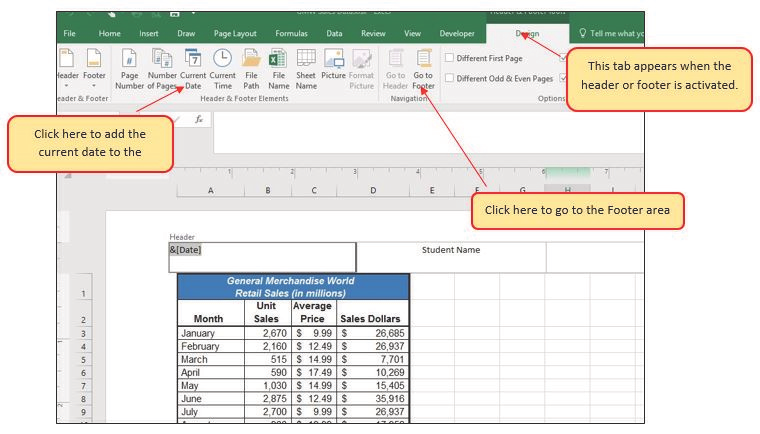
\includegraphics[width=\maxwidth{.95\linewidth}]{gfx/ch01_fig50}
	\caption{Tab for Creating Headers and Footers}
	\label{01:fig50}
\end{figure}

\begin{enumerate}[resume]
	\item Type the author's name in the center section of the Header.
	\item Click in the left section of the Header (see Figure \ref{01:fig50}).
	\item Click \fmtButton{Design $ \Rightarrow $ Header \& Footer Elements $ \Rightarrow $ Current Date}. Note: the date will display as \textit{\&[Date]} until the workbook is printed or the normal view is restored.
	\item Click \fmtButton{Design $ \Rightarrow $ Navigation $ \Rightarrow $ Go To Footer}.
	\item Click in the right section of the footer.
	\item Click \fmtButton{Design $ \Rightarrow $ Header \& Footer $ \Rightarrow $ Page Number}. Note: the page number will display as \textit{\&[Page]} until the workbook is printed or the normal view is restored.
	\item Click any cell location outside the header or footer area.
	\item Click the \fmtButton{Normal} view button in the lower right side of the Status Bar (see Figure \ref{01:fig51}).

\end{enumerate}

\begin{figure}[H]
	\centering
	\includegraphics[width=\maxwidth{.95\linewidth}]{gfx/ch01_fig51}
	\caption{Worksheet in Page Layout View}
	\label{01:fig51}
\end{figure}

\subsection{Printing Worksheets and Workbooks}

Once the print settings have been adjusted and the headers and footers added, it is time to print the worksheet. The following steps explain how to print the worksheet in the \textit{CH1-GMW Sales} workbook.

\begin{enumerate}
	\item Click the \fmtButton{File} tab on the Ribbon.
	\item Click the \fmtButton{Print} option on the left side of the \textit{Backstage} view (see Figure \ref{01:fig52}). Notice that there is a preview of the printed worksheet on the right side of the \textit{Backstage} view.
\end{enumerate}

\begin{figure}[H]
	\centering
	\includegraphics[width=\maxwidth{.95\linewidth}]{gfx/ch01_fig52}
	\caption{Backstage View Print option}
	\label{01:fig52}
\end{figure}

\begin{enumerate}[resume]
	\item Click the \fmtButton{Print Active Sheets} button in the \fmtButton{Print} section of the \textit{Backstage} view (see Figure \ref{01:fig52}).
	\item Click the \fmtButton{Print} button to print the active sheet.
	\item Click the \fmtButton{Home} tab of the Ribbon.
	\item Save and close the \fmtWorksheet{CH1-GMW Sales} workbook.
	\item Compare the worksheet with the self-check answer key (\fmtWorksheet{CH1-GMW Sales Data Soln}) and then submit the \fmtWorksheet{CH1-GMW Sales} workbook as directed by the instructor.
\end{enumerate}

\begin{center}
	\begin{tkwbox}{Key Take-Aways}
		\textbf{Print}
		\\
		\begin{itemize}
			\setlength{\itemsep}{0pt}
			\setlength{\parskip}{0pt}
			\setlength{\parsep}{0pt}

			\item The commands in the Page Layout tab of the Ribbon are used to prepare a worksheet for printing.
			\item Headers and footers can be added to a worksheet to show key information such as page numbers, the date, the file name, author's name, and so on.
			\item The \fmtButton{Print} commands are in the \fmtButton{File} tab of the Ribbon.
			
		\end{itemize}
	\end{tkwbox}
\end{center}

\section{Chapter Practice}

\subsection{Basic Monthly Budget for a Medical Office}

Creating and maintaining budgets are common practices in many careers. Budgets play a critical role in helping a business or household control expenditures. In this exercise a budget for a hypothetical medical office will be created while reviewing the skills covered in this chapter.

\begin{enumerate}
	\item Open the file named \fmtWorksheet{PR1-Data}, then save as \fmtWorksheet{PR1-Medical Office Budget}.
	\item Activate all the cell locations in the \fmtWorksheet{Sheet1} worksheet by clicking the \fmtButton{Select All} button in the upper left corner of the worksheet (See Figure \ref{01:fig53}).
\end{enumerate}

\begin{figure}[H]
	\centering
	\includegraphics[width=\maxwidth{.95\linewidth}]{gfx/ch01_fig53}
	\caption{The Select All Button}
	\label{01:fig53}
\end{figure}

\begin{enumerate}[resume]
	\item In the \fmtButton{Home} tab of the Ribbon, set the font style to Arial and the font size to $ 12 $ points. Then click any cell to deselect the worksheet.
	\item Double-click the divider between the tops of \fmtLoc{Column A} and \fmtLoc{Column B} to automatically change the width of \fmtLoc{Column A} so all the entries in the range \fmtLoc{A3:A8} are visible. 
	\item Click in \fmtLoc{B2} and enter \fmtTyping{Quarter 1}.
	\item Use the \fmtButton{Auto Fill Handle} to complete the headings in the range \fmtLoc{C2:E2}. Click in cell \fmtLoc{B2} and place the mouse pointer over the \fmtButton{Auto Fill Handle}. When the mouse pointer changes to a black plus sign, left click and drag it to cell \fmtLoc{E2}.
	\item Click \fmtLoc{B2:E2} to select those cells. 
	\item Click \fmtButton{Home $ \Rightarrow $ Cells $ \Rightarrow $ Format $ \Rightarrow $ Column Width}. Set the column width to $ 11.57 $.
	\item Click \fmtLoc{A1} and enter \fmtTyping{Medical Office Budget}.
	\item Click on \fmtLoc{B1} and then click \fmtButton{Home $ \Rightarrow $ Cells $ \Rightarrow $ Insert $ \Rightarrow $ Insert Sheet Columns}.
	\item Click \fmtLoc{B2} and enter \fmtTyping{Budget Cost}.
	\item Adjust the width of \fmtLoc{Column B} to approximately $ 13.25 $ characters.
	\item Click-and-drag from \fmtLoc{A1} to \fmtLoc{F1} to select that range. 
	\item Click \fmtButton{Home $ \Rightarrow $ Alignment $ \Rightarrow $ Merge \& Center}.
	\item Make the following format adjustments to the merged range \fmtLoc{A1:F1}: bold; italics; change the font size to $ 14 $ points; change the cell fill color to Aqua-Accent $ 5 $-Darker $ 50 $\%, and change the font color to white.
	\item Click \fmtLoc{A1} then click \fmtButton{Home $ \Rightarrow $ Cells $ \Rightarrow $ Format $ \Rightarrow $ Row Height}. Set the height to $ 24.75 $.
	\item Make the following format adjustment to the range \fmtLoc{A2:F2}: bold; fill color to Tan-Background $ 2 $-Darker $ 10 $\%. Center the column titles so that they are horizontally centered in each cell.
	\item Select \fmtLoc{B2} and then click \fmtButton{Home $ \Rightarrow $ Alignment $ \Rightarrow $ Wrap Text}. 
	\item Copy cell \fmtLoc{C3} and paste the contents into the range \fmtLoc{D3:F3}.
	\item Click \fmtLoc{C6} and drag to \fmtLoc{C8} to select that range. Click \fmtButton{Home $ \Rightarrow $ Clipboard $ \Rightarrow $ Copy}.
	\item Click \fmtLoc{D6} and drag to \fmtLoc{F8} to select that range. Click \fmtButton{Home $ \Rightarrow $ Clipboard $ \Rightarrow $ Paste}.
	\item Click cell \fmtLoc{B3}. Click \fmtButton{Formulas $ \Rightarrow $ Function Library $ \Rightarrow $ AutoSum}. To complete the formula, click \fmtLoc{C3} and drag to \fmtLoc{F3} to select that range, then press the \fmtKeystroke{Enter} key.
	\item Copy the formula in cell \fmtLoc{B3} and paste it into the range \fmtLoc{B4:B8}.
	\item Format the range \fmtLoc{B3:F8} with Accounting format and zero decimal places.
	\item Select the range \fmtLoc{A1:F8}.
	\item Click \fmtButton{Home $ \Rightarrow $ Font $ \Rightarrow $ Borders}. Select \fmtButton{All Borders}.
	\item Double click the \fmtWorksheet{Sheet1} tab at the bottom of the worksheet and change its name to \fmtTyping{Budget}, then press the \fmtKeystroke{Enter} key. 
	\item Delete all unused worksheets.
	\item Click \fmtButton{Page Layout $ \Rightarrow $ Page Setup $ \Rightarrow $ Orientation $ \Rightarrow $ Landscape}.
	\item Add a header to the \fmtWorksheet{Budget} worksheet that shows the current date in the upper left corner and the author's name in the center.
	\item Add a footer to the \fmtWorksheet{Budget} worksheet that shows the page number in the lower right corner. 
	\item Save the \fmtWorksheet{PR1-Medical Office Budget} workbook.
	\item Compare the worksheet with the self-check answer key and then submit the \fmtWorksheet{PR1-Medical Office Budget} workbook as directed by the instructor.
\end{enumerate}

\section{Scored Assessment}

\subsection{Sales and Inventory Items}

A key activity for marketing professionals is to analyze projected sales and inventory information. This is especially important for retail environments. This exercise utilizes the skills covered in this chapter to analyze sales and inventory data.

\begin{enumerate}
	\item Open the file named \fmtWorksheet{SC1-Data} and then save as \fmtWorksheet{SC1-Sales and Inventory}
	\item In the \fmtWorksheet{Sheet1} worksheet, enter the word \fmtTyping{Totals} in cell \fmtLoc{C14}.
	\item Format all the cells in \fmtWorksheet{Sheet1} to Century font style and a 12-point font size.
	\item Set the column width for \fmtLoc{Column A} through \fmtLoc{Column G} to $ 13.5 $.
	\item Edit the entry in cell \fmtLoc{B2} to read \fmtTyping{Item Number}.
	\item Use the \fmtButton{Auto Fill Handle} to fill the Item Numbers from \fmtLoc{B3} into the range \fmtLoc{B4:B13}. The item numbers should increase by one as they are filled through the range so \fmtLoc{B13} is $ A1510 $.
	\item Copy the content of cell \fmtLoc{A3} and paste it into the range \fmtLoc{A4:A8}.
	\item Delete \fmtLoc{Column F}.
	\item Format the range \fmtLoc{A1:F2} so the text is Bold.
	\item Set the alignment in the range \fmtLoc{A2:F2} to Wrap Text.
	\item Prepare \fmtLoc{A1:F1} for the title text by changing the fill color of the cells in the range \fmtLoc{A1:F1} to Red, Accent $ 2 $, Darker 25\%.
	\item Make the following font changes to the range \fmtLoc{A1:F1}: set the font color to white, add italics, and set the font size to $ 14 $.
	\item Merge and center the cells in the range \fmtLoc{A1:F1}.
	\item Enter the title for this worksheet in the range \fmtLoc{A1:F1}. The title should appear on two lines. The first line should read \fmtTyping{Status Report} and the second line should read \fmtTyping{Sales and Inventory by Item}.
	\item Increase the height of \fmtLoc{Row $ 1 $} so the entire title is visible.
	\item Format the values in the range \fmtLoc{C3:C13} with dollar signs and two decimal places.
	\item Format the values in the range \fmtLoc{E3:F13} with comma style, zero decimal places.
	\item In cell \fmtLoc{E14}, use \fmtButton{AutoSum} to calculate the sum of the values in the range \fmtLoc{E3:E13}.
	\item In cell \fmtLoc{F14}, use \fmtButton{AutoSum} to calculate the sum of the values in the range \fmtLoc{F3:F13}.
	\item Apply \fmtButton{All Borders} to the range \fmtLoc{A1:F14}.
	\item Add a thick bottom border to \fmtLoc{A2:F2}; add a thick bottom border to \fmtLoc{A13:F13}.
	\item Add a thick outside border around the perimeter of the range \fmtLoc{A1:F14}.
	\item Insert a new blank worksheet in the workbook (this will be \fmtWorksheet{Sheet4}).
	\item Delete \fmtWorksheet{Sheet3}.
	\item Move \fmtWorksheet{Sheet4} ahead of \fmtWorksheet{Sheet2} so the order of the worksheets is \fmtWorksheet{Sheet1}, \fmtWorksheet{Sheet4}, and \fmtWorksheet{Sheet2}.
	\item Rename the \fmtWorksheet{Sheet1} worksheet tab to \fmtTyping{Status Report}.
	\item Change the orientation of the \fmtWorksheet{Status Report} worksheet so it prints landscape instead of portrait.
	\item Add a header to the \fmtWorksheet{Status Report} worksheet that shows the date in the upper left corner and the author's name in the center.
	\item Add a footer to the \fmtWorksheet{Status Report} worksheet that shows the page number in the lower right corner with the word \textit{Page} before the number.
	\item Center the worksheet both horizontally and vertically on the sheet.
	\item Save the \fmtWorksheet{SC1-Sales and Inventory} workbook.
	\item Submit the \fmtWorksheet{SC1-Sales and Inventory} workbook as directed by the instructor.

\end{enumerate}
